% Created by tikzDevice version 0.12.6 on 2026-09-14 08:46:32
% !TEX encoding = UTF-8 Unicode
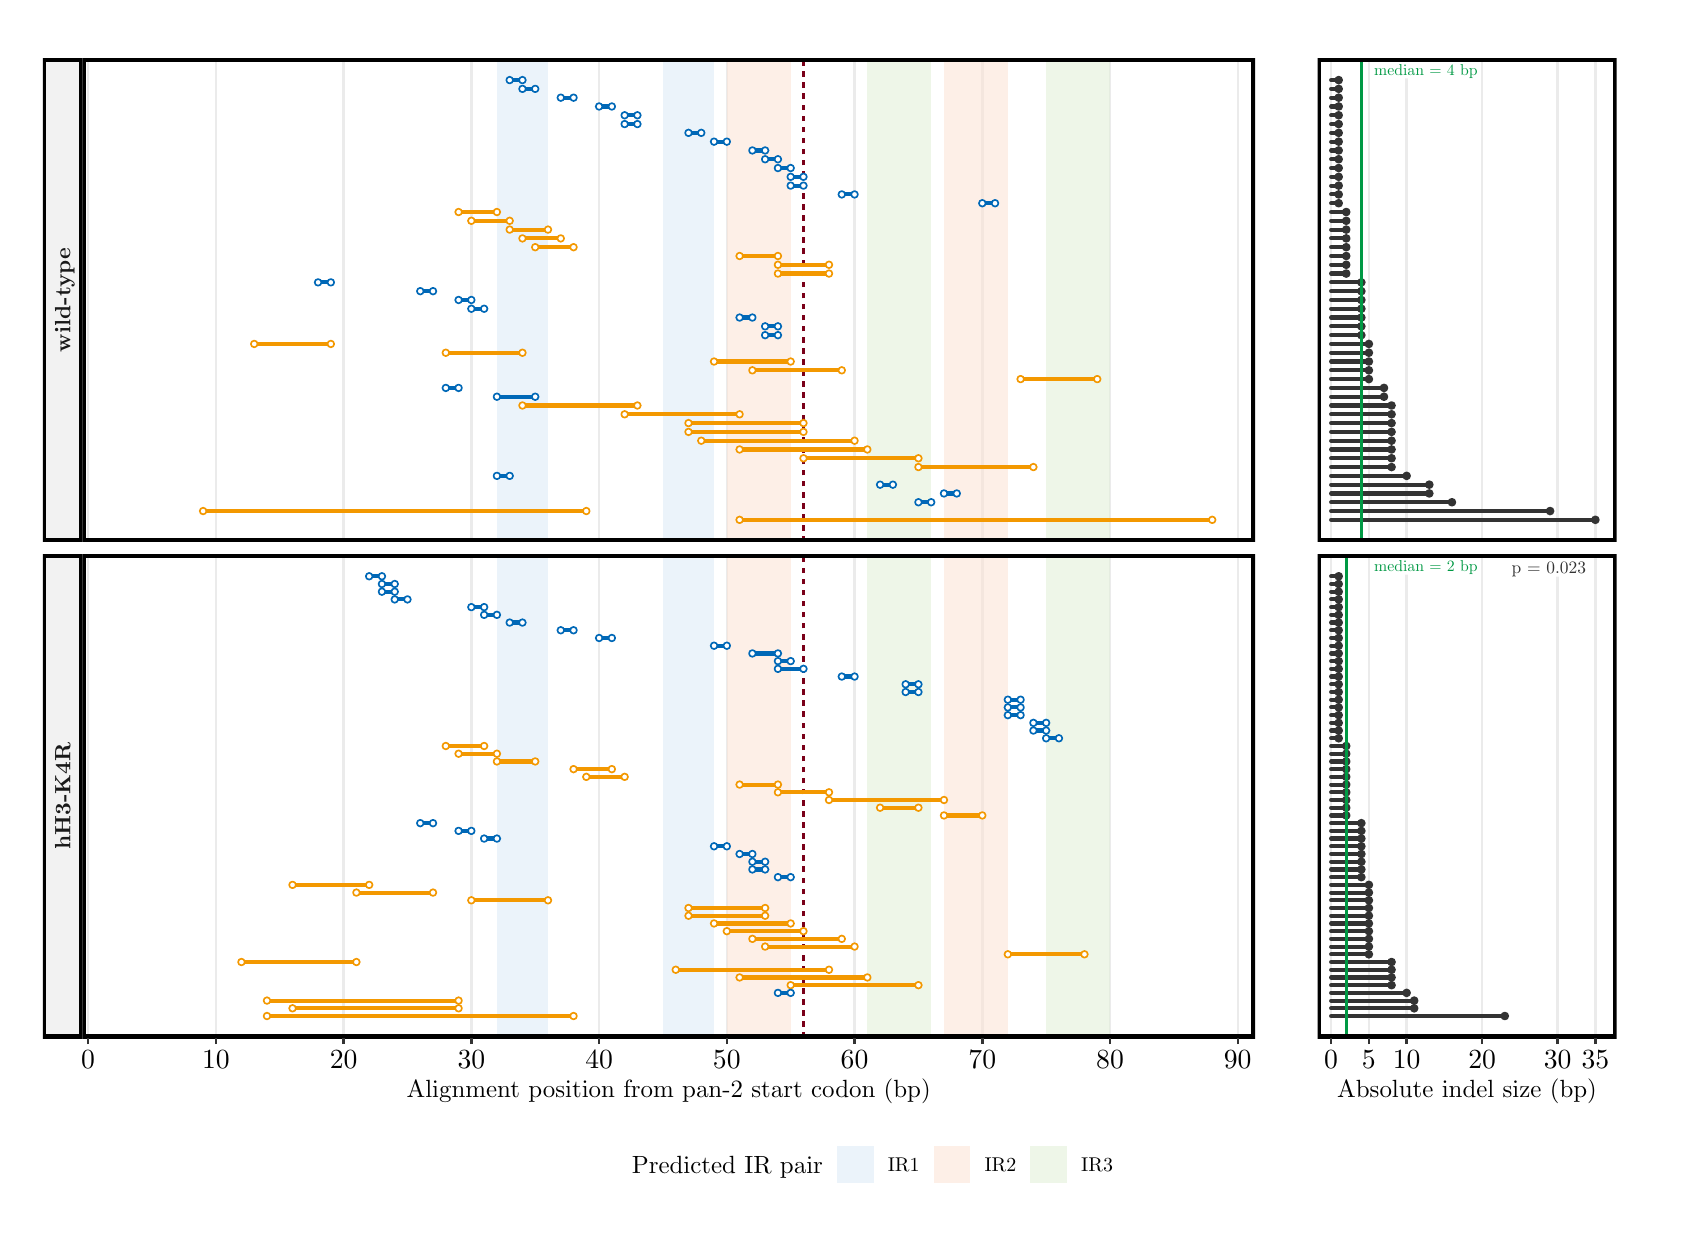
\begin{tikzpicture}[x=1pt,y=1pt]
\definecolor{fillColor}{RGB}{255,255,255}
\path[use as bounding box,fill=fillColor,fill opacity=0.00] (0,0) rectangle (596.23,433.62);
\begin{scope}
\path[clip] (  0.00,  0.00) rectangle (596.23,433.62);
\definecolor{drawColor}{RGB}{255,255,255}
\definecolor{fillColor}{RGB}{255,255,255}

\path[draw=drawColor,line width= 1.1pt,line join=round,line cap=round,fill=fillColor] (  0.00,  0.00) rectangle (596.23,433.62);
\end{scope}
\begin{scope}
\path[clip] (  5.50,  5.50) rectangle (446.49,428.12);
\definecolor{drawColor}{RGB}{255,255,255}
\definecolor{fillColor}{RGB}{255,255,255}

\path[draw=drawColor,line width= 0.9pt,line join=round,line cap=round,fill=fillColor] (  5.50,  5.50) rectangle (446.49,428.12);
\end{scope}
\begin{scope}
\path[clip] (446.49,  5.50) rectangle (590.73,428.12);
\definecolor{drawColor}{RGB}{255,255,255}
\definecolor{fillColor}{RGB}{255,255,255}

\path[draw=drawColor,line width= 0.9pt,line join=round,line cap=round,fill=fillColor] (446.49,  5.50) rectangle (590.73,428.12);
\end{scope}
\begin{scope}
\path[clip] ( 19.78,247.83) rectangle (443.49,422.62);
\definecolor{fillColor}{RGB}{255,255,255}

\path[fill=fillColor] ( 19.78,247.83) rectangle (443.49,422.62);
\definecolor{drawColor}{gray}{0.92}

\path[draw=drawColor,line width= 0.9pt,line join=round] ( 21.85,247.83) --
	( 21.85,422.62);

\path[draw=drawColor,line width= 0.9pt,line join=round] ( 68.01,247.83) --
	( 68.01,422.62);

\path[draw=drawColor,line width= 0.9pt,line join=round] (114.17,247.83) --
	(114.17,422.62);

\path[draw=drawColor,line width= 0.9pt,line join=round] (160.32,247.83) --
	(160.32,422.62);

\path[draw=drawColor,line width= 0.9pt,line join=round] (206.48,247.83) --
	(206.48,422.62);

\path[draw=drawColor,line width= 0.9pt,line join=round] (252.63,247.83) --
	(252.63,422.62);

\path[draw=drawColor,line width= 0.9pt,line join=round] (298.79,247.83) --
	(298.79,422.62);

\path[draw=drawColor,line width= 0.9pt,line join=round] (344.95,247.83) --
	(344.95,422.62);

\path[draw=drawColor,line width= 0.9pt,line join=round] (391.10,247.83) --
	(391.10,422.62);

\path[draw=drawColor,line width= 0.9pt,line join=round] (437.26,247.83) --
	(437.26,422.62);
\definecolor{fillColor}{RGB}{221,235,247}

\path[fill=fillColor,fill opacity=0.58] (169.55,247.83) rectangle (188.02,422.62);

\path[fill=fillColor,fill opacity=0.58] (229.56,247.83) rectangle (248.02,422.62);
\definecolor{fillColor}{RGB}{252,228,214}

\path[fill=fillColor,fill opacity=0.58] (252.63,247.83) rectangle (275.71,422.62);

\path[fill=fillColor,fill opacity=0.58] (331.10,247.83) rectangle (354.18,422.62);
\definecolor{fillColor}{RGB}{226,240,217}

\path[fill=fillColor,fill opacity=0.58] (303.41,247.83) rectangle (326.48,422.62);

\path[fill=fillColor,fill opacity=0.58] (368.02,247.83) rectangle (391.10,422.62);
\definecolor{drawColor}{RGB}{122,0,25}

\path[draw=drawColor,line width= 0.9pt,dash pattern=on 2pt off 2pt ,line join=round] (280.33,247.83) -- (280.33,422.62);
\definecolor{drawColor}{RGB}{0,104,183}

\path[draw=drawColor,line width= 1.5pt,line join=round,line cap=round] (174.17,414.67) -- (178.78,414.67);

\path[draw=drawColor,line width= 1.5pt,line join=round,line cap=round] (178.78,411.50) -- (183.40,411.50);

\path[draw=drawColor,line width= 1.5pt,line join=round,line cap=round] (192.63,408.32) -- (197.25,408.32);

\path[draw=drawColor,line width= 1.5pt,line join=round,line cap=round] (206.48,405.14) -- (211.09,405.14);

\path[draw=drawColor,line width= 1.5pt,line join=round,line cap=round] (215.71,401.96) -- (220.32,401.96);

\path[draw=drawColor,line width= 1.5pt,line join=round,line cap=round] (215.71,398.78) -- (220.32,398.78);

\path[draw=drawColor,line width= 1.5pt,line join=round,line cap=round] (238.79,395.61) -- (243.40,395.61);

\path[draw=drawColor,line width= 1.5pt,line join=round,line cap=round] (248.02,392.43) -- (252.63,392.43);

\path[draw=drawColor,line width= 1.5pt,line join=round,line cap=round] (261.87,389.25) -- (266.48,389.25);

\path[draw=drawColor,line width= 1.5pt,line join=round,line cap=round] (266.48,386.07) -- (271.10,386.07);

\path[draw=drawColor,line width= 1.5pt,line join=round,line cap=round] (271.10,382.89) -- (275.71,382.89);

\path[draw=drawColor,line width= 1.5pt,line join=round,line cap=round] (275.71,379.72) -- (280.33,379.72);

\path[draw=drawColor,line width= 1.5pt,line join=round,line cap=round] (275.71,376.54) -- (280.33,376.54);

\path[draw=drawColor,line width= 1.5pt,line join=round,line cap=round] (294.17,373.36) -- (298.79,373.36);

\path[draw=drawColor,line width= 1.5pt,line join=round,line cap=round] (344.95,370.18) -- (349.56,370.18);
\definecolor{drawColor}{RGB}{243,152,0}

\path[draw=drawColor,line width= 1.5pt,line join=round,line cap=round] (155.71,367.00) -- (169.55,367.00);

\path[draw=drawColor,line width= 1.5pt,line join=round,line cap=round] (160.32,363.83) -- (174.17,363.83);

\path[draw=drawColor,line width= 1.5pt,line join=round,line cap=round] (174.17,360.65) -- (188.02,360.65);

\path[draw=drawColor,line width= 1.5pt,line join=round,line cap=round] (178.78,357.47) -- (192.63,357.47);

\path[draw=drawColor,line width= 1.5pt,line join=round,line cap=round] (183.40,354.29) -- (197.25,354.29);

\path[draw=drawColor,line width= 1.5pt,line join=round,line cap=round] (257.25,351.11) -- (271.10,351.11);

\path[draw=drawColor,line width= 1.5pt,line join=round,line cap=round] (271.10,347.94) -- (289.56,347.94);

\path[draw=drawColor,line width= 1.5pt,line join=round,line cap=round] (271.10,344.76) -- (289.56,344.76);
\definecolor{drawColor}{RGB}{0,104,183}

\path[draw=drawColor,line width= 1.5pt,line join=round,line cap=round] (104.93,341.58) -- (109.55,341.58);

\path[draw=drawColor,line width= 1.5pt,line join=round,line cap=round] (141.86,338.40) -- (146.47,338.40);

\path[draw=drawColor,line width= 1.5pt,line join=round,line cap=round] (155.71,335.22) -- (160.32,335.22);

\path[draw=drawColor,line width= 1.5pt,line join=round,line cap=round] (160.32,332.05) -- (164.94,332.05);

\path[draw=drawColor,line width= 1.5pt,line join=round,line cap=round] (257.25,328.87) -- (261.87,328.87);

\path[draw=drawColor,line width= 1.5pt,line join=round,line cap=round] (266.48,325.69) -- (271.10,325.69);

\path[draw=drawColor,line width= 1.5pt,line join=round,line cap=round] (266.48,322.51) -- (271.10,322.51);
\definecolor{drawColor}{RGB}{243,152,0}

\path[draw=drawColor,line width= 1.5pt,line join=round,line cap=round] ( 81.86,319.33) -- (109.55,319.33);

\path[draw=drawColor,line width= 1.5pt,line join=round,line cap=round] (151.09,316.15) -- (178.78,316.15);

\path[draw=drawColor,line width= 1.5pt,line join=round,line cap=round] (248.02,312.98) -- (275.71,312.98);

\path[draw=drawColor,line width= 1.5pt,line join=round,line cap=round] (261.87,309.80) -- (294.17,309.80);

\path[draw=drawColor,line width= 1.5pt,line join=round,line cap=round] (358.79,306.62) -- (386.49,306.62);
\definecolor{drawColor}{RGB}{0,104,183}

\path[draw=drawColor,line width= 1.5pt,line join=round,line cap=round] (151.09,303.44) -- (155.71,303.44);

\path[draw=drawColor,line width= 1.5pt,line join=round,line cap=round] (169.55,300.26) -- (183.40,300.26);
\definecolor{drawColor}{RGB}{243,152,0}

\path[draw=drawColor,line width= 1.5pt,line join=round,line cap=round] (178.78,297.09) -- (220.32,297.09);

\path[draw=drawColor,line width= 1.5pt,line join=round,line cap=round] (215.71,293.91) -- (257.25,293.91);

\path[draw=drawColor,line width= 1.5pt,line join=round,line cap=round] (238.79,290.73) -- (280.33,290.73);

\path[draw=drawColor,line width= 1.5pt,line join=round,line cap=round] (238.79,287.55) -- (280.33,287.55);

\path[draw=drawColor,line width= 1.5pt,line join=round,line cap=round] (243.40,284.37) -- (298.79,284.37);

\path[draw=drawColor,line width= 1.5pt,line join=round,line cap=round] (257.25,281.20) -- (303.41,281.20);

\path[draw=drawColor,line width= 1.5pt,line join=round,line cap=round] (280.33,278.02) -- (321.87,278.02);

\path[draw=drawColor,line width= 1.5pt,line join=round,line cap=round] (321.87,274.84) -- (363.41,274.84);
\definecolor{drawColor}{RGB}{0,104,183}

\path[draw=drawColor,line width= 1.5pt,line join=round,line cap=round] (169.55,271.66) -- (174.17,271.66);

\path[draw=drawColor,line width= 1.5pt,line join=round,line cap=round] (308.02,268.48) -- (312.64,268.48);

\path[draw=drawColor,line width= 1.5pt,line join=round,line cap=round] (331.10,265.31) -- (335.72,265.31);

\path[draw=drawColor,line width= 1.5pt,line join=round,line cap=round] (321.87,262.13) -- (326.48,262.13);
\definecolor{drawColor}{RGB}{243,152,0}

\path[draw=drawColor,line width= 1.5pt,line join=round,line cap=round] ( 63.39,258.95) -- (201.86,258.95);

\path[draw=drawColor,line width= 1.5pt,line join=round,line cap=round] (257.25,255.77) -- (428.03,255.77);
\definecolor{drawColor}{RGB}{0,104,183}
\definecolor{fillColor}{RGB}{255,255,255}

\path[draw=drawColor,line width= 0.6pt,line join=round,line cap=round,fill=fillColor] (174.17,414.67) circle (  1.21);

\path[draw=drawColor,line width= 0.6pt,line join=round,line cap=round,fill=fillColor] (178.78,411.50) circle (  1.21);

\path[draw=drawColor,line width= 0.6pt,line join=round,line cap=round,fill=fillColor] (192.63,408.32) circle (  1.21);

\path[draw=drawColor,line width= 0.6pt,line join=round,line cap=round,fill=fillColor] (206.48,405.14) circle (  1.21);

\path[draw=drawColor,line width= 0.6pt,line join=round,line cap=round,fill=fillColor] (215.71,401.96) circle (  1.21);

\path[draw=drawColor,line width= 0.6pt,line join=round,line cap=round,fill=fillColor] (215.71,398.78) circle (  1.21);

\path[draw=drawColor,line width= 0.6pt,line join=round,line cap=round,fill=fillColor] (238.79,395.61) circle (  1.21);

\path[draw=drawColor,line width= 0.6pt,line join=round,line cap=round,fill=fillColor] (248.02,392.43) circle (  1.21);

\path[draw=drawColor,line width= 0.6pt,line join=round,line cap=round,fill=fillColor] (261.87,389.25) circle (  1.21);

\path[draw=drawColor,line width= 0.6pt,line join=round,line cap=round,fill=fillColor] (266.48,386.07) circle (  1.21);

\path[draw=drawColor,line width= 0.6pt,line join=round,line cap=round,fill=fillColor] (271.10,382.89) circle (  1.21);

\path[draw=drawColor,line width= 0.6pt,line join=round,line cap=round,fill=fillColor] (275.71,379.72) circle (  1.21);

\path[draw=drawColor,line width= 0.6pt,line join=round,line cap=round,fill=fillColor] (275.71,376.54) circle (  1.21);

\path[draw=drawColor,line width= 0.6pt,line join=round,line cap=round,fill=fillColor] (294.17,373.36) circle (  1.21);

\path[draw=drawColor,line width= 0.6pt,line join=round,line cap=round,fill=fillColor] (344.95,370.18) circle (  1.21);
\definecolor{drawColor}{RGB}{243,152,0}

\path[draw=drawColor,line width= 0.6pt,line join=round,line cap=round,fill=fillColor] (155.71,367.00) circle (  1.21);

\path[draw=drawColor,line width= 0.6pt,line join=round,line cap=round,fill=fillColor] (160.32,363.83) circle (  1.21);

\path[draw=drawColor,line width= 0.6pt,line join=round,line cap=round,fill=fillColor] (174.17,360.65) circle (  1.21);

\path[draw=drawColor,line width= 0.6pt,line join=round,line cap=round,fill=fillColor] (178.78,357.47) circle (  1.21);

\path[draw=drawColor,line width= 0.6pt,line join=round,line cap=round,fill=fillColor] (183.40,354.29) circle (  1.21);

\path[draw=drawColor,line width= 0.6pt,line join=round,line cap=round,fill=fillColor] (257.25,351.11) circle (  1.21);

\path[draw=drawColor,line width= 0.6pt,line join=round,line cap=round,fill=fillColor] (271.10,347.94) circle (  1.21);

\path[draw=drawColor,line width= 0.6pt,line join=round,line cap=round,fill=fillColor] (271.10,344.76) circle (  1.21);
\definecolor{drawColor}{RGB}{0,104,183}

\path[draw=drawColor,line width= 0.6pt,line join=round,line cap=round,fill=fillColor] (104.93,341.58) circle (  1.21);

\path[draw=drawColor,line width= 0.6pt,line join=round,line cap=round,fill=fillColor] (141.86,338.40) circle (  1.21);

\path[draw=drawColor,line width= 0.6pt,line join=round,line cap=round,fill=fillColor] (155.71,335.22) circle (  1.21);

\path[draw=drawColor,line width= 0.6pt,line join=round,line cap=round,fill=fillColor] (160.32,332.05) circle (  1.21);

\path[draw=drawColor,line width= 0.6pt,line join=round,line cap=round,fill=fillColor] (257.25,328.87) circle (  1.21);

\path[draw=drawColor,line width= 0.6pt,line join=round,line cap=round,fill=fillColor] (266.48,325.69) circle (  1.21);

\path[draw=drawColor,line width= 0.6pt,line join=round,line cap=round,fill=fillColor] (266.48,322.51) circle (  1.21);
\definecolor{drawColor}{RGB}{243,152,0}

\path[draw=drawColor,line width= 0.6pt,line join=round,line cap=round,fill=fillColor] ( 81.86,319.33) circle (  1.21);

\path[draw=drawColor,line width= 0.6pt,line join=round,line cap=round,fill=fillColor] (151.09,316.15) circle (  1.21);

\path[draw=drawColor,line width= 0.6pt,line join=round,line cap=round,fill=fillColor] (248.02,312.98) circle (  1.21);

\path[draw=drawColor,line width= 0.6pt,line join=round,line cap=round,fill=fillColor] (261.87,309.80) circle (  1.21);

\path[draw=drawColor,line width= 0.6pt,line join=round,line cap=round,fill=fillColor] (358.79,306.62) circle (  1.21);
\definecolor{drawColor}{RGB}{0,104,183}

\path[draw=drawColor,line width= 0.6pt,line join=round,line cap=round,fill=fillColor] (151.09,303.44) circle (  1.21);

\path[draw=drawColor,line width= 0.6pt,line join=round,line cap=round,fill=fillColor] (169.55,300.26) circle (  1.21);
\definecolor{drawColor}{RGB}{243,152,0}

\path[draw=drawColor,line width= 0.6pt,line join=round,line cap=round,fill=fillColor] (178.78,297.09) circle (  1.21);

\path[draw=drawColor,line width= 0.6pt,line join=round,line cap=round,fill=fillColor] (215.71,293.91) circle (  1.21);

\path[draw=drawColor,line width= 0.6pt,line join=round,line cap=round,fill=fillColor] (238.79,290.73) circle (  1.21);

\path[draw=drawColor,line width= 0.6pt,line join=round,line cap=round,fill=fillColor] (238.79,287.55) circle (  1.21);

\path[draw=drawColor,line width= 0.6pt,line join=round,line cap=round,fill=fillColor] (243.40,284.37) circle (  1.21);

\path[draw=drawColor,line width= 0.6pt,line join=round,line cap=round,fill=fillColor] (257.25,281.20) circle (  1.21);

\path[draw=drawColor,line width= 0.6pt,line join=round,line cap=round,fill=fillColor] (280.33,278.02) circle (  1.21);

\path[draw=drawColor,line width= 0.6pt,line join=round,line cap=round,fill=fillColor] (321.87,274.84) circle (  1.21);
\definecolor{drawColor}{RGB}{0,104,183}

\path[draw=drawColor,line width= 0.6pt,line join=round,line cap=round,fill=fillColor] (169.55,271.66) circle (  1.21);

\path[draw=drawColor,line width= 0.6pt,line join=round,line cap=round,fill=fillColor] (308.02,268.48) circle (  1.21);

\path[draw=drawColor,line width= 0.6pt,line join=round,line cap=round,fill=fillColor] (331.10,265.31) circle (  1.21);

\path[draw=drawColor,line width= 0.6pt,line join=round,line cap=round,fill=fillColor] (321.87,262.13) circle (  1.21);
\definecolor{drawColor}{RGB}{243,152,0}

\path[draw=drawColor,line width= 0.6pt,line join=round,line cap=round,fill=fillColor] ( 63.39,258.95) circle (  1.21);

\path[draw=drawColor,line width= 0.6pt,line join=round,line cap=round,fill=fillColor] (257.25,255.77) circle (  1.21);
\definecolor{drawColor}{RGB}{0,104,183}

\path[draw=drawColor,line width= 0.6pt,line join=round,line cap=round,fill=fillColor] (178.78,414.67) circle (  1.21);

\path[draw=drawColor,line width= 0.6pt,line join=round,line cap=round,fill=fillColor] (183.40,411.50) circle (  1.21);

\path[draw=drawColor,line width= 0.6pt,line join=round,line cap=round,fill=fillColor] (197.25,408.32) circle (  1.21);

\path[draw=drawColor,line width= 0.6pt,line join=round,line cap=round,fill=fillColor] (211.09,405.14) circle (  1.21);

\path[draw=drawColor,line width= 0.6pt,line join=round,line cap=round,fill=fillColor] (220.32,401.96) circle (  1.21);

\path[draw=drawColor,line width= 0.6pt,line join=round,line cap=round,fill=fillColor] (220.32,398.78) circle (  1.21);

\path[draw=drawColor,line width= 0.6pt,line join=round,line cap=round,fill=fillColor] (243.40,395.61) circle (  1.21);

\path[draw=drawColor,line width= 0.6pt,line join=round,line cap=round,fill=fillColor] (252.63,392.43) circle (  1.21);

\path[draw=drawColor,line width= 0.6pt,line join=round,line cap=round,fill=fillColor] (266.48,389.25) circle (  1.21);

\path[draw=drawColor,line width= 0.6pt,line join=round,line cap=round,fill=fillColor] (271.10,386.07) circle (  1.21);

\path[draw=drawColor,line width= 0.6pt,line join=round,line cap=round,fill=fillColor] (275.71,382.89) circle (  1.21);

\path[draw=drawColor,line width= 0.6pt,line join=round,line cap=round,fill=fillColor] (280.33,379.72) circle (  1.21);

\path[draw=drawColor,line width= 0.6pt,line join=round,line cap=round,fill=fillColor] (280.33,376.54) circle (  1.21);

\path[draw=drawColor,line width= 0.6pt,line join=round,line cap=round,fill=fillColor] (298.79,373.36) circle (  1.21);

\path[draw=drawColor,line width= 0.6pt,line join=round,line cap=round,fill=fillColor] (349.56,370.18) circle (  1.21);
\definecolor{drawColor}{RGB}{243,152,0}

\path[draw=drawColor,line width= 0.6pt,line join=round,line cap=round,fill=fillColor] (169.55,367.00) circle (  1.21);

\path[draw=drawColor,line width= 0.6pt,line join=round,line cap=round,fill=fillColor] (174.17,363.83) circle (  1.21);

\path[draw=drawColor,line width= 0.6pt,line join=round,line cap=round,fill=fillColor] (188.02,360.65) circle (  1.21);

\path[draw=drawColor,line width= 0.6pt,line join=round,line cap=round,fill=fillColor] (192.63,357.47) circle (  1.21);

\path[draw=drawColor,line width= 0.6pt,line join=round,line cap=round,fill=fillColor] (197.25,354.29) circle (  1.21);

\path[draw=drawColor,line width= 0.6pt,line join=round,line cap=round,fill=fillColor] (271.10,351.11) circle (  1.21);

\path[draw=drawColor,line width= 0.6pt,line join=round,line cap=round,fill=fillColor] (289.56,347.94) circle (  1.21);

\path[draw=drawColor,line width= 0.6pt,line join=round,line cap=round,fill=fillColor] (289.56,344.76) circle (  1.21);
\definecolor{drawColor}{RGB}{0,104,183}

\path[draw=drawColor,line width= 0.6pt,line join=round,line cap=round,fill=fillColor] (109.55,341.58) circle (  1.21);

\path[draw=drawColor,line width= 0.6pt,line join=round,line cap=round,fill=fillColor] (146.47,338.40) circle (  1.21);

\path[draw=drawColor,line width= 0.6pt,line join=round,line cap=round,fill=fillColor] (160.32,335.22) circle (  1.21);

\path[draw=drawColor,line width= 0.6pt,line join=round,line cap=round,fill=fillColor] (164.94,332.05) circle (  1.21);

\path[draw=drawColor,line width= 0.6pt,line join=round,line cap=round,fill=fillColor] (261.87,328.87) circle (  1.21);

\path[draw=drawColor,line width= 0.6pt,line join=round,line cap=round,fill=fillColor] (271.10,325.69) circle (  1.21);

\path[draw=drawColor,line width= 0.6pt,line join=round,line cap=round,fill=fillColor] (271.10,322.51) circle (  1.21);
\definecolor{drawColor}{RGB}{243,152,0}

\path[draw=drawColor,line width= 0.6pt,line join=round,line cap=round,fill=fillColor] (109.55,319.33) circle (  1.21);

\path[draw=drawColor,line width= 0.6pt,line join=round,line cap=round,fill=fillColor] (178.78,316.15) circle (  1.21);

\path[draw=drawColor,line width= 0.6pt,line join=round,line cap=round,fill=fillColor] (275.71,312.98) circle (  1.21);

\path[draw=drawColor,line width= 0.6pt,line join=round,line cap=round,fill=fillColor] (294.17,309.80) circle (  1.21);

\path[draw=drawColor,line width= 0.6pt,line join=round,line cap=round,fill=fillColor] (386.49,306.62) circle (  1.21);
\definecolor{drawColor}{RGB}{0,104,183}

\path[draw=drawColor,line width= 0.6pt,line join=round,line cap=round,fill=fillColor] (155.71,303.44) circle (  1.21);

\path[draw=drawColor,line width= 0.6pt,line join=round,line cap=round,fill=fillColor] (183.40,300.26) circle (  1.21);
\definecolor{drawColor}{RGB}{243,152,0}

\path[draw=drawColor,line width= 0.6pt,line join=round,line cap=round,fill=fillColor] (220.32,297.09) circle (  1.21);

\path[draw=drawColor,line width= 0.6pt,line join=round,line cap=round,fill=fillColor] (257.25,293.91) circle (  1.21);

\path[draw=drawColor,line width= 0.6pt,line join=round,line cap=round,fill=fillColor] (280.33,290.73) circle (  1.21);

\path[draw=drawColor,line width= 0.6pt,line join=round,line cap=round,fill=fillColor] (280.33,287.55) circle (  1.21);

\path[draw=drawColor,line width= 0.6pt,line join=round,line cap=round,fill=fillColor] (298.79,284.37) circle (  1.21);

\path[draw=drawColor,line width= 0.6pt,line join=round,line cap=round,fill=fillColor] (303.41,281.20) circle (  1.21);

\path[draw=drawColor,line width= 0.6pt,line join=round,line cap=round,fill=fillColor] (321.87,278.02) circle (  1.21);

\path[draw=drawColor,line width= 0.6pt,line join=round,line cap=round,fill=fillColor] (363.41,274.84) circle (  1.21);
\definecolor{drawColor}{RGB}{0,104,183}

\path[draw=drawColor,line width= 0.6pt,line join=round,line cap=round,fill=fillColor] (174.17,271.66) circle (  1.21);

\path[draw=drawColor,line width= 0.6pt,line join=round,line cap=round,fill=fillColor] (312.64,268.48) circle (  1.21);

\path[draw=drawColor,line width= 0.6pt,line join=round,line cap=round,fill=fillColor] (335.72,265.31) circle (  1.21);

\path[draw=drawColor,line width= 0.6pt,line join=round,line cap=round,fill=fillColor] (326.48,262.13) circle (  1.21);
\definecolor{drawColor}{RGB}{243,152,0}

\path[draw=drawColor,line width= 0.6pt,line join=round,line cap=round,fill=fillColor] (201.86,258.95) circle (  1.21);

\path[draw=drawColor,line width= 0.6pt,line join=round,line cap=round,fill=fillColor] (428.03,255.77) circle (  1.21);
\definecolor{drawColor}{RGB}{0,0,0}

\path[draw=drawColor,line width= 2.6pt,line join=round,line cap=round] ( 19.78,247.83) rectangle (443.49,422.62);
\end{scope}
\begin{scope}
\path[clip] ( 19.78, 68.53) rectangle (443.49,243.33);
\definecolor{fillColor}{RGB}{255,255,255}

\path[fill=fillColor] ( 19.78, 68.53) rectangle (443.49,243.33);
\definecolor{drawColor}{gray}{0.92}

\path[draw=drawColor,line width= 0.9pt,line join=round] ( 21.85, 68.53) --
	( 21.85,243.33);

\path[draw=drawColor,line width= 0.9pt,line join=round] ( 68.01, 68.53) --
	( 68.01,243.33);

\path[draw=drawColor,line width= 0.9pt,line join=round] (114.17, 68.53) --
	(114.17,243.33);

\path[draw=drawColor,line width= 0.9pt,line join=round] (160.32, 68.53) --
	(160.32,243.33);

\path[draw=drawColor,line width= 0.9pt,line join=round] (206.48, 68.53) --
	(206.48,243.33);

\path[draw=drawColor,line width= 0.9pt,line join=round] (252.63, 68.53) --
	(252.63,243.33);

\path[draw=drawColor,line width= 0.9pt,line join=round] (298.79, 68.53) --
	(298.79,243.33);

\path[draw=drawColor,line width= 0.9pt,line join=round] (344.95, 68.53) --
	(344.95,243.33);

\path[draw=drawColor,line width= 0.9pt,line join=round] (391.10, 68.53) --
	(391.10,243.33);

\path[draw=drawColor,line width= 0.9pt,line join=round] (437.26, 68.53) --
	(437.26,243.33);
\definecolor{fillColor}{RGB}{221,235,247}

\path[fill=fillColor,fill opacity=0.58] (169.55, 68.53) rectangle (188.02,243.33);

\path[fill=fillColor,fill opacity=0.58] (229.56, 68.53) rectangle (248.02,243.33);
\definecolor{fillColor}{RGB}{252,228,214}

\path[fill=fillColor,fill opacity=0.58] (252.63, 68.53) rectangle (275.71,243.33);

\path[fill=fillColor,fill opacity=0.58] (331.10, 68.53) rectangle (354.18,243.33);
\definecolor{fillColor}{RGB}{226,240,217}

\path[fill=fillColor,fill opacity=0.58] (303.41, 68.53) rectangle (326.48,243.33);

\path[fill=fillColor,fill opacity=0.58] (368.02, 68.53) rectangle (391.10,243.33);
\definecolor{drawColor}{RGB}{122,0,25}

\path[draw=drawColor,line width= 0.9pt,dash pattern=on 2pt off 2pt ,line join=round] (280.33, 68.53) -- (280.33,243.33);
\definecolor{drawColor}{RGB}{0,104,183}

\path[draw=drawColor,line width= 1.5pt,line join=round,line cap=round] (123.40,235.38) -- (128.01,235.38);

\path[draw=drawColor,line width= 1.5pt,line join=round,line cap=round] (128.01,232.59) -- (132.63,232.59);

\path[draw=drawColor,line width= 1.5pt,line join=round,line cap=round] (128.01,229.81) -- (132.63,229.81);

\path[draw=drawColor,line width= 1.5pt,line join=round,line cap=round] (132.63,227.02) -- (137.24,227.02);

\path[draw=drawColor,line width= 1.5pt,line join=round,line cap=round] (160.32,224.23) -- (164.94,224.23);

\path[draw=drawColor,line width= 1.5pt,line join=round,line cap=round] (164.94,221.44) -- (169.55,221.44);

\path[draw=drawColor,line width= 1.5pt,line join=round,line cap=round] (174.17,218.65) -- (178.78,218.65);

\path[draw=drawColor,line width= 1.5pt,line join=round,line cap=round] (192.63,215.87) -- (197.25,215.87);

\path[draw=drawColor,line width= 1.5pt,line join=round,line cap=round] (206.48,213.08) -- (211.09,213.08);

\path[draw=drawColor,line width= 1.5pt,line join=round,line cap=round] (248.02,210.29) -- (252.63,210.29);

\path[draw=drawColor,line width= 1.5pt,line join=round,line cap=round] (261.87,207.50) -- (271.10,207.50);

\path[draw=drawColor,line width= 1.5pt,line join=round,line cap=round] (271.10,204.72) -- (275.71,204.72);

\path[draw=drawColor,line width= 1.5pt,line join=round,line cap=round] (271.10,201.93) -- (280.33,201.93);

\path[draw=drawColor,line width= 1.5pt,line join=round,line cap=round] (294.17,199.14) -- (298.79,199.14);

\path[draw=drawColor,line width= 1.5pt,line join=round,line cap=round] (317.25,196.35) -- (321.87,196.35);

\path[draw=drawColor,line width= 1.5pt,line join=round,line cap=round] (317.25,193.56) -- (321.87,193.56);

\path[draw=drawColor,line width= 1.5pt,line join=round,line cap=round] (354.18,190.78) -- (358.79,190.78);

\path[draw=drawColor,line width= 1.5pt,line join=round,line cap=round] (354.18,187.99) -- (358.79,187.99);

\path[draw=drawColor,line width= 1.5pt,line join=round,line cap=round] (354.18,185.20) -- (358.79,185.20);

\path[draw=drawColor,line width= 1.5pt,line join=round,line cap=round] (363.41,182.41) -- (368.02,182.41);

\path[draw=drawColor,line width= 1.5pt,line join=round,line cap=round] (363.41,179.63) -- (368.02,179.63);

\path[draw=drawColor,line width= 1.5pt,line join=round,line cap=round] (368.02,176.84) -- (372.64,176.84);
\definecolor{drawColor}{RGB}{243,152,0}

\path[draw=drawColor,line width= 1.5pt,line join=round,line cap=round] (151.09,174.05) -- (164.94,174.05);

\path[draw=drawColor,line width= 1.5pt,line join=round,line cap=round] (155.71,171.26) -- (169.55,171.26);

\path[draw=drawColor,line width= 1.5pt,line join=round,line cap=round] (169.55,168.47) -- (183.40,168.47);

\path[draw=drawColor,line width= 1.5pt,line join=round,line cap=round] (197.25,165.69) -- (211.09,165.69);

\path[draw=drawColor,line width= 1.5pt,line join=round,line cap=round] (201.86,162.90) -- (215.71,162.90);

\path[draw=drawColor,line width= 1.5pt,line join=round,line cap=round] (257.25,160.11) -- (271.10,160.11);

\path[draw=drawColor,line width= 1.5pt,line join=round,line cap=round] (271.10,157.32) -- (289.56,157.32);

\path[draw=drawColor,line width= 1.5pt,line join=round,line cap=round] (289.56,154.54) -- (331.10,154.54);

\path[draw=drawColor,line width= 1.5pt,line join=round,line cap=round] (308.02,151.75) -- (321.87,151.75);

\path[draw=drawColor,line width= 1.5pt,line join=round,line cap=round] (331.10,148.96) -- (344.95,148.96);
\definecolor{drawColor}{RGB}{0,104,183}

\path[draw=drawColor,line width= 1.5pt,line join=round,line cap=round] (141.86,146.17) -- (146.47,146.17);

\path[draw=drawColor,line width= 1.5pt,line join=round,line cap=round] (155.71,143.38) -- (160.32,143.38);

\path[draw=drawColor,line width= 1.5pt,line join=round,line cap=round] (164.94,140.60) -- (169.55,140.60);

\path[draw=drawColor,line width= 1.5pt,line join=round,line cap=round] (248.02,137.81) -- (252.63,137.81);

\path[draw=drawColor,line width= 1.5pt,line join=round,line cap=round] (257.25,135.02) -- (261.87,135.02);

\path[draw=drawColor,line width= 1.5pt,line join=round,line cap=round] (261.87,132.23) -- (266.48,132.23);

\path[draw=drawColor,line width= 1.5pt,line join=round,line cap=round] (261.87,129.45) -- (266.48,129.45);

\path[draw=drawColor,line width= 1.5pt,line join=round,line cap=round] (271.10,126.66) -- (275.71,126.66);
\definecolor{drawColor}{RGB}{243,152,0}

\path[draw=drawColor,line width= 1.5pt,line join=round,line cap=round] ( 95.70,123.87) -- (123.40,123.87);

\path[draw=drawColor,line width= 1.5pt,line join=round,line cap=round] (118.78,121.08) -- (146.47,121.08);

\path[draw=drawColor,line width= 1.5pt,line join=round,line cap=round] (160.32,118.29) -- (188.02,118.29);

\path[draw=drawColor,line width= 1.5pt,line join=round,line cap=round] (238.79,115.51) -- (266.48,115.51);

\path[draw=drawColor,line width= 1.5pt,line join=round,line cap=round] (238.79,112.72) -- (266.48,112.72);

\path[draw=drawColor,line width= 1.5pt,line join=round,line cap=round] (248.02,109.93) -- (275.71,109.93);

\path[draw=drawColor,line width= 1.5pt,line join=round,line cap=round] (252.63,107.14) -- (280.33,107.14);

\path[draw=drawColor,line width= 1.5pt,line join=round,line cap=round] (261.87,104.36) -- (294.17,104.36);

\path[draw=drawColor,line width= 1.5pt,line join=round,line cap=round] (266.48,101.57) -- (298.79,101.57);

\path[draw=drawColor,line width= 1.5pt,line join=round,line cap=round] (354.18, 98.78) -- (381.87, 98.78);

\path[draw=drawColor,line width= 1.5pt,line join=round,line cap=round] ( 77.24, 95.99) -- (118.78, 95.99);

\path[draw=drawColor,line width= 1.5pt,line join=round,line cap=round] (234.17, 93.20) -- (289.56, 93.20);

\path[draw=drawColor,line width= 1.5pt,line join=round,line cap=round] (257.25, 90.42) -- (303.41, 90.42);

\path[draw=drawColor,line width= 1.5pt,line join=round,line cap=round] (275.71, 87.63) -- (321.87, 87.63);
\definecolor{drawColor}{RGB}{0,104,183}

\path[draw=drawColor,line width= 1.5pt,line join=round,line cap=round] (271.10, 84.84) -- (275.71, 84.84);
\definecolor{drawColor}{RGB}{243,152,0}

\path[draw=drawColor,line width= 1.5pt,line join=round,line cap=round] ( 86.47, 82.05) -- (155.71, 82.05);

\path[draw=drawColor,line width= 1.5pt,line join=round,line cap=round] ( 95.70, 79.27) -- (155.71, 79.27);

\path[draw=drawColor,line width= 1.5pt,line join=round,line cap=round] ( 86.47, 76.48) -- (197.25, 76.48);
\definecolor{drawColor}{RGB}{0,104,183}
\definecolor{fillColor}{RGB}{255,255,255}

\path[draw=drawColor,line width= 0.6pt,line join=round,line cap=round,fill=fillColor] (123.40,235.38) circle (  1.21);

\path[draw=drawColor,line width= 0.6pt,line join=round,line cap=round,fill=fillColor] (128.01,232.59) circle (  1.21);

\path[draw=drawColor,line width= 0.6pt,line join=round,line cap=round,fill=fillColor] (128.01,229.81) circle (  1.21);

\path[draw=drawColor,line width= 0.6pt,line join=round,line cap=round,fill=fillColor] (132.63,227.02) circle (  1.21);

\path[draw=drawColor,line width= 0.6pt,line join=round,line cap=round,fill=fillColor] (160.32,224.23) circle (  1.21);

\path[draw=drawColor,line width= 0.6pt,line join=round,line cap=round,fill=fillColor] (164.94,221.44) circle (  1.21);

\path[draw=drawColor,line width= 0.6pt,line join=round,line cap=round,fill=fillColor] (174.17,218.65) circle (  1.21);

\path[draw=drawColor,line width= 0.6pt,line join=round,line cap=round,fill=fillColor] (192.63,215.87) circle (  1.21);

\path[draw=drawColor,line width= 0.6pt,line join=round,line cap=round,fill=fillColor] (206.48,213.08) circle (  1.21);

\path[draw=drawColor,line width= 0.6pt,line join=round,line cap=round,fill=fillColor] (248.02,210.29) circle (  1.21);

\path[draw=drawColor,line width= 0.6pt,line join=round,line cap=round,fill=fillColor] (261.87,207.50) circle (  1.21);

\path[draw=drawColor,line width= 0.6pt,line join=round,line cap=round,fill=fillColor] (271.10,204.72) circle (  1.21);

\path[draw=drawColor,line width= 0.6pt,line join=round,line cap=round,fill=fillColor] (271.10,201.93) circle (  1.21);

\path[draw=drawColor,line width= 0.6pt,line join=round,line cap=round,fill=fillColor] (294.17,199.14) circle (  1.21);

\path[draw=drawColor,line width= 0.6pt,line join=round,line cap=round,fill=fillColor] (317.25,196.35) circle (  1.21);

\path[draw=drawColor,line width= 0.6pt,line join=round,line cap=round,fill=fillColor] (317.25,193.56) circle (  1.21);

\path[draw=drawColor,line width= 0.6pt,line join=round,line cap=round,fill=fillColor] (354.18,190.78) circle (  1.21);

\path[draw=drawColor,line width= 0.6pt,line join=round,line cap=round,fill=fillColor] (354.18,187.99) circle (  1.21);

\path[draw=drawColor,line width= 0.6pt,line join=round,line cap=round,fill=fillColor] (354.18,185.20) circle (  1.21);

\path[draw=drawColor,line width= 0.6pt,line join=round,line cap=round,fill=fillColor] (363.41,182.41) circle (  1.21);

\path[draw=drawColor,line width= 0.6pt,line join=round,line cap=round,fill=fillColor] (363.41,179.63) circle (  1.21);

\path[draw=drawColor,line width= 0.6pt,line join=round,line cap=round,fill=fillColor] (368.02,176.84) circle (  1.21);
\definecolor{drawColor}{RGB}{243,152,0}

\path[draw=drawColor,line width= 0.6pt,line join=round,line cap=round,fill=fillColor] (151.09,174.05) circle (  1.21);

\path[draw=drawColor,line width= 0.6pt,line join=round,line cap=round,fill=fillColor] (155.71,171.26) circle (  1.21);

\path[draw=drawColor,line width= 0.6pt,line join=round,line cap=round,fill=fillColor] (169.55,168.47) circle (  1.21);

\path[draw=drawColor,line width= 0.6pt,line join=round,line cap=round,fill=fillColor] (197.25,165.69) circle (  1.21);

\path[draw=drawColor,line width= 0.6pt,line join=round,line cap=round,fill=fillColor] (201.86,162.90) circle (  1.21);

\path[draw=drawColor,line width= 0.6pt,line join=round,line cap=round,fill=fillColor] (257.25,160.11) circle (  1.21);

\path[draw=drawColor,line width= 0.6pt,line join=round,line cap=round,fill=fillColor] (271.10,157.32) circle (  1.21);

\path[draw=drawColor,line width= 0.6pt,line join=round,line cap=round,fill=fillColor] (289.56,154.54) circle (  1.21);

\path[draw=drawColor,line width= 0.6pt,line join=round,line cap=round,fill=fillColor] (308.02,151.75) circle (  1.21);

\path[draw=drawColor,line width= 0.6pt,line join=round,line cap=round,fill=fillColor] (331.10,148.96) circle (  1.21);
\definecolor{drawColor}{RGB}{0,104,183}

\path[draw=drawColor,line width= 0.6pt,line join=round,line cap=round,fill=fillColor] (141.86,146.17) circle (  1.21);

\path[draw=drawColor,line width= 0.6pt,line join=round,line cap=round,fill=fillColor] (155.71,143.38) circle (  1.21);

\path[draw=drawColor,line width= 0.6pt,line join=round,line cap=round,fill=fillColor] (164.94,140.60) circle (  1.21);

\path[draw=drawColor,line width= 0.6pt,line join=round,line cap=round,fill=fillColor] (248.02,137.81) circle (  1.21);

\path[draw=drawColor,line width= 0.6pt,line join=round,line cap=round,fill=fillColor] (257.25,135.02) circle (  1.21);

\path[draw=drawColor,line width= 0.6pt,line join=round,line cap=round,fill=fillColor] (261.87,132.23) circle (  1.21);

\path[draw=drawColor,line width= 0.6pt,line join=round,line cap=round,fill=fillColor] (261.87,129.45) circle (  1.21);

\path[draw=drawColor,line width= 0.6pt,line join=round,line cap=round,fill=fillColor] (271.10,126.66) circle (  1.21);
\definecolor{drawColor}{RGB}{243,152,0}

\path[draw=drawColor,line width= 0.6pt,line join=round,line cap=round,fill=fillColor] ( 95.70,123.87) circle (  1.21);

\path[draw=drawColor,line width= 0.6pt,line join=round,line cap=round,fill=fillColor] (118.78,121.08) circle (  1.21);

\path[draw=drawColor,line width= 0.6pt,line join=round,line cap=round,fill=fillColor] (160.32,118.29) circle (  1.21);

\path[draw=drawColor,line width= 0.6pt,line join=round,line cap=round,fill=fillColor] (238.79,115.51) circle (  1.21);

\path[draw=drawColor,line width= 0.6pt,line join=round,line cap=round,fill=fillColor] (238.79,112.72) circle (  1.21);

\path[draw=drawColor,line width= 0.6pt,line join=round,line cap=round,fill=fillColor] (248.02,109.93) circle (  1.21);

\path[draw=drawColor,line width= 0.6pt,line join=round,line cap=round,fill=fillColor] (252.63,107.14) circle (  1.21);

\path[draw=drawColor,line width= 0.6pt,line join=round,line cap=round,fill=fillColor] (261.87,104.36) circle (  1.21);

\path[draw=drawColor,line width= 0.6pt,line join=round,line cap=round,fill=fillColor] (266.48,101.57) circle (  1.21);

\path[draw=drawColor,line width= 0.6pt,line join=round,line cap=round,fill=fillColor] (354.18, 98.78) circle (  1.21);

\path[draw=drawColor,line width= 0.6pt,line join=round,line cap=round,fill=fillColor] ( 77.24, 95.99) circle (  1.21);

\path[draw=drawColor,line width= 0.6pt,line join=round,line cap=round,fill=fillColor] (234.17, 93.20) circle (  1.21);

\path[draw=drawColor,line width= 0.6pt,line join=round,line cap=round,fill=fillColor] (257.25, 90.42) circle (  1.21);

\path[draw=drawColor,line width= 0.6pt,line join=round,line cap=round,fill=fillColor] (275.71, 87.63) circle (  1.21);
\definecolor{drawColor}{RGB}{0,104,183}

\path[draw=drawColor,line width= 0.6pt,line join=round,line cap=round,fill=fillColor] (271.10, 84.84) circle (  1.21);
\definecolor{drawColor}{RGB}{243,152,0}

\path[draw=drawColor,line width= 0.6pt,line join=round,line cap=round,fill=fillColor] ( 86.47, 82.05) circle (  1.21);

\path[draw=drawColor,line width= 0.6pt,line join=round,line cap=round,fill=fillColor] ( 95.70, 79.27) circle (  1.21);

\path[draw=drawColor,line width= 0.6pt,line join=round,line cap=round,fill=fillColor] ( 86.47, 76.48) circle (  1.21);
\definecolor{drawColor}{RGB}{0,104,183}

\path[draw=drawColor,line width= 0.6pt,line join=round,line cap=round,fill=fillColor] (128.01,235.38) circle (  1.21);

\path[draw=drawColor,line width= 0.6pt,line join=round,line cap=round,fill=fillColor] (132.63,232.59) circle (  1.21);

\path[draw=drawColor,line width= 0.6pt,line join=round,line cap=round,fill=fillColor] (132.63,229.81) circle (  1.21);

\path[draw=drawColor,line width= 0.6pt,line join=round,line cap=round,fill=fillColor] (137.24,227.02) circle (  1.21);

\path[draw=drawColor,line width= 0.6pt,line join=round,line cap=round,fill=fillColor] (164.94,224.23) circle (  1.21);

\path[draw=drawColor,line width= 0.6pt,line join=round,line cap=round,fill=fillColor] (169.55,221.44) circle (  1.21);

\path[draw=drawColor,line width= 0.6pt,line join=round,line cap=round,fill=fillColor] (178.78,218.65) circle (  1.21);

\path[draw=drawColor,line width= 0.6pt,line join=round,line cap=round,fill=fillColor] (197.25,215.87) circle (  1.21);

\path[draw=drawColor,line width= 0.6pt,line join=round,line cap=round,fill=fillColor] (211.09,213.08) circle (  1.21);

\path[draw=drawColor,line width= 0.6pt,line join=round,line cap=round,fill=fillColor] (252.63,210.29) circle (  1.21);

\path[draw=drawColor,line width= 0.6pt,line join=round,line cap=round,fill=fillColor] (271.10,207.50) circle (  1.21);

\path[draw=drawColor,line width= 0.6pt,line join=round,line cap=round,fill=fillColor] (275.71,204.72) circle (  1.21);

\path[draw=drawColor,line width= 0.6pt,line join=round,line cap=round,fill=fillColor] (280.33,201.93) circle (  1.21);

\path[draw=drawColor,line width= 0.6pt,line join=round,line cap=round,fill=fillColor] (298.79,199.14) circle (  1.21);

\path[draw=drawColor,line width= 0.6pt,line join=round,line cap=round,fill=fillColor] (321.87,196.35) circle (  1.21);

\path[draw=drawColor,line width= 0.6pt,line join=round,line cap=round,fill=fillColor] (321.87,193.56) circle (  1.21);

\path[draw=drawColor,line width= 0.6pt,line join=round,line cap=round,fill=fillColor] (358.79,190.78) circle (  1.21);

\path[draw=drawColor,line width= 0.6pt,line join=round,line cap=round,fill=fillColor] (358.79,187.99) circle (  1.21);

\path[draw=drawColor,line width= 0.6pt,line join=round,line cap=round,fill=fillColor] (358.79,185.20) circle (  1.21);

\path[draw=drawColor,line width= 0.6pt,line join=round,line cap=round,fill=fillColor] (368.02,182.41) circle (  1.21);

\path[draw=drawColor,line width= 0.6pt,line join=round,line cap=round,fill=fillColor] (368.02,179.63) circle (  1.21);

\path[draw=drawColor,line width= 0.6pt,line join=round,line cap=round,fill=fillColor] (372.64,176.84) circle (  1.21);
\definecolor{drawColor}{RGB}{243,152,0}

\path[draw=drawColor,line width= 0.6pt,line join=round,line cap=round,fill=fillColor] (164.94,174.05) circle (  1.21);

\path[draw=drawColor,line width= 0.6pt,line join=round,line cap=round,fill=fillColor] (169.55,171.26) circle (  1.21);

\path[draw=drawColor,line width= 0.6pt,line join=round,line cap=round,fill=fillColor] (183.40,168.47) circle (  1.21);

\path[draw=drawColor,line width= 0.6pt,line join=round,line cap=round,fill=fillColor] (211.09,165.69) circle (  1.21);

\path[draw=drawColor,line width= 0.6pt,line join=round,line cap=round,fill=fillColor] (215.71,162.90) circle (  1.21);

\path[draw=drawColor,line width= 0.6pt,line join=round,line cap=round,fill=fillColor] (271.10,160.11) circle (  1.21);

\path[draw=drawColor,line width= 0.6pt,line join=round,line cap=round,fill=fillColor] (289.56,157.32) circle (  1.21);

\path[draw=drawColor,line width= 0.6pt,line join=round,line cap=round,fill=fillColor] (331.10,154.54) circle (  1.21);

\path[draw=drawColor,line width= 0.6pt,line join=round,line cap=round,fill=fillColor] (321.87,151.75) circle (  1.21);

\path[draw=drawColor,line width= 0.6pt,line join=round,line cap=round,fill=fillColor] (344.95,148.96) circle (  1.21);
\definecolor{drawColor}{RGB}{0,104,183}

\path[draw=drawColor,line width= 0.6pt,line join=round,line cap=round,fill=fillColor] (146.47,146.17) circle (  1.21);

\path[draw=drawColor,line width= 0.6pt,line join=round,line cap=round,fill=fillColor] (160.32,143.38) circle (  1.21);

\path[draw=drawColor,line width= 0.6pt,line join=round,line cap=round,fill=fillColor] (169.55,140.60) circle (  1.21);

\path[draw=drawColor,line width= 0.6pt,line join=round,line cap=round,fill=fillColor] (252.63,137.81) circle (  1.21);

\path[draw=drawColor,line width= 0.6pt,line join=round,line cap=round,fill=fillColor] (261.87,135.02) circle (  1.21);

\path[draw=drawColor,line width= 0.6pt,line join=round,line cap=round,fill=fillColor] (266.48,132.23) circle (  1.21);

\path[draw=drawColor,line width= 0.6pt,line join=round,line cap=round,fill=fillColor] (266.48,129.45) circle (  1.21);

\path[draw=drawColor,line width= 0.6pt,line join=round,line cap=round,fill=fillColor] (275.71,126.66) circle (  1.21);
\definecolor{drawColor}{RGB}{243,152,0}

\path[draw=drawColor,line width= 0.6pt,line join=round,line cap=round,fill=fillColor] (123.40,123.87) circle (  1.21);

\path[draw=drawColor,line width= 0.6pt,line join=round,line cap=round,fill=fillColor] (146.47,121.08) circle (  1.21);

\path[draw=drawColor,line width= 0.6pt,line join=round,line cap=round,fill=fillColor] (188.02,118.29) circle (  1.21);

\path[draw=drawColor,line width= 0.6pt,line join=round,line cap=round,fill=fillColor] (266.48,115.51) circle (  1.21);

\path[draw=drawColor,line width= 0.6pt,line join=round,line cap=round,fill=fillColor] (266.48,112.72) circle (  1.21);

\path[draw=drawColor,line width= 0.6pt,line join=round,line cap=round,fill=fillColor] (275.71,109.93) circle (  1.21);

\path[draw=drawColor,line width= 0.6pt,line join=round,line cap=round,fill=fillColor] (280.33,107.14) circle (  1.21);

\path[draw=drawColor,line width= 0.6pt,line join=round,line cap=round,fill=fillColor] (294.17,104.36) circle (  1.21);

\path[draw=drawColor,line width= 0.6pt,line join=round,line cap=round,fill=fillColor] (298.79,101.57) circle (  1.21);

\path[draw=drawColor,line width= 0.6pt,line join=round,line cap=round,fill=fillColor] (381.87, 98.78) circle (  1.21);

\path[draw=drawColor,line width= 0.6pt,line join=round,line cap=round,fill=fillColor] (118.78, 95.99) circle (  1.21);

\path[draw=drawColor,line width= 0.6pt,line join=round,line cap=round,fill=fillColor] (289.56, 93.20) circle (  1.21);

\path[draw=drawColor,line width= 0.6pt,line join=round,line cap=round,fill=fillColor] (303.41, 90.42) circle (  1.21);

\path[draw=drawColor,line width= 0.6pt,line join=round,line cap=round,fill=fillColor] (321.87, 87.63) circle (  1.21);
\definecolor{drawColor}{RGB}{0,104,183}

\path[draw=drawColor,line width= 0.6pt,line join=round,line cap=round,fill=fillColor] (275.71, 84.84) circle (  1.21);
\definecolor{drawColor}{RGB}{243,152,0}

\path[draw=drawColor,line width= 0.6pt,line join=round,line cap=round,fill=fillColor] (155.71, 82.05) circle (  1.21);

\path[draw=drawColor,line width= 0.6pt,line join=round,line cap=round,fill=fillColor] (155.71, 79.27) circle (  1.21);

\path[draw=drawColor,line width= 0.6pt,line join=round,line cap=round,fill=fillColor] (197.25, 76.48) circle (  1.21);
\definecolor{drawColor}{RGB}{0,0,0}

\path[draw=drawColor,line width= 2.6pt,line join=round,line cap=round] ( 19.78, 68.53) rectangle (443.49,243.33);
\end{scope}
\begin{scope}
\path[clip] (  5.50,247.83) rectangle ( 19.78,422.62);
\definecolor{drawColor}{RGB}{0,0,0}
\definecolor{fillColor}{gray}{0.95}

\path[draw=drawColor,line width= 2.6pt,line join=round,line cap=round,fill=fillColor] (  5.50,247.83) rectangle ( 19.78,422.62);
\definecolor{drawColor}{gray}{0.10}

\node[text=drawColor,rotate= 90.00,anchor=base,inner sep=0pt, outer sep=0pt, scale=  0.80] at ( 15.40,335.22) {\bfseries wild-type};
\end{scope}
\begin{scope}
\path[clip] (  5.50, 68.53) rectangle ( 19.78,243.33);
\definecolor{drawColor}{RGB}{0,0,0}
\definecolor{fillColor}{gray}{0.95}

\path[draw=drawColor,line width= 2.6pt,line join=round,line cap=round,fill=fillColor] (  5.50, 68.53) rectangle ( 19.78,243.33);
\definecolor{drawColor}{gray}{0.10}

\node[text=drawColor,rotate= 90.00,anchor=base,inner sep=0pt, outer sep=0pt, scale=  0.80] at ( 15.40,155.93) {\bfseries hH3-K4R};
\end{scope}
\begin{scope}
\path[clip] (  0.00,  0.00) rectangle (596.23,433.62);
\definecolor{drawColor}{gray}{0.20}

\path[draw=drawColor,line width= 0.9pt,line join=round] ( 21.85, 66.28) --
	( 21.85, 68.53);

\path[draw=drawColor,line width= 0.9pt,line join=round] ( 68.01, 66.28) --
	( 68.01, 68.53);

\path[draw=drawColor,line width= 0.9pt,line join=round] (114.17, 66.28) --
	(114.17, 68.53);

\path[draw=drawColor,line width= 0.9pt,line join=round] (160.32, 66.28) --
	(160.32, 68.53);

\path[draw=drawColor,line width= 0.9pt,line join=round] (206.48, 66.28) --
	(206.48, 68.53);

\path[draw=drawColor,line width= 0.9pt,line join=round] (252.63, 66.28) --
	(252.63, 68.53);

\path[draw=drawColor,line width= 0.9pt,line join=round] (298.79, 66.28) --
	(298.79, 68.53);

\path[draw=drawColor,line width= 0.9pt,line join=round] (344.95, 66.28) --
	(344.95, 68.53);

\path[draw=drawColor,line width= 0.9pt,line join=round] (391.10, 66.28) --
	(391.10, 68.53);

\path[draw=drawColor,line width= 0.9pt,line join=round] (437.26, 66.28) --
	(437.26, 68.53);
\end{scope}
\begin{scope}
\path[clip] (  0.00,  0.00) rectangle (596.23,433.62);
\definecolor{drawColor}{RGB}{0,0,0}

\node[text=drawColor,anchor=base,inner sep=0pt, outer sep=0pt, scale=  1.00] at ( 21.85, 57.60) {0};

\node[text=drawColor,anchor=base,inner sep=0pt, outer sep=0pt, scale=  1.00] at ( 68.01, 57.60) {10};

\node[text=drawColor,anchor=base,inner sep=0pt, outer sep=0pt, scale=  1.00] at (114.17, 57.60) {20};

\node[text=drawColor,anchor=base,inner sep=0pt, outer sep=0pt, scale=  1.00] at (160.32, 57.60) {30};

\node[text=drawColor,anchor=base,inner sep=0pt, outer sep=0pt, scale=  1.00] at (206.48, 57.60) {40};

\node[text=drawColor,anchor=base,inner sep=0pt, outer sep=0pt, scale=  1.00] at (252.63, 57.60) {50};

\node[text=drawColor,anchor=base,inner sep=0pt, outer sep=0pt, scale=  1.00] at (298.79, 57.60) {60};

\node[text=drawColor,anchor=base,inner sep=0pt, outer sep=0pt, scale=  1.00] at (344.95, 57.60) {70};

\node[text=drawColor,anchor=base,inner sep=0pt, outer sep=0pt, scale=  1.00] at (391.10, 57.60) {80};

\node[text=drawColor,anchor=base,inner sep=0pt, outer sep=0pt, scale=  1.00] at (437.26, 57.60) {90};
\end{scope}
\begin{scope}
\path[clip] (  0.00,  0.00) rectangle (596.23,433.62);
\definecolor{drawColor}{RGB}{0,0,0}

\node[text=drawColor,anchor=base,inner sep=0pt, outer sep=0pt, scale=  0.90] at (231.63, 47.20) {Alignment position from pan-2 start codon (bp)};
\end{scope}
\begin{scope}
\path[clip] (466.09,247.83) rectangle (574.12,422.62);
\definecolor{fillColor}{RGB}{255,255,255}

\path[fill=fillColor] (466.09,247.83) rectangle (574.12,422.62);
\definecolor{drawColor}{gray}{0.92}

\path[draw=drawColor,line width= 0.9pt,line join=round] (471.00,247.83) --
	(471.00,422.62);

\path[draw=drawColor,line width= 0.9pt,line join=round] (484.64,247.83) --
	(484.64,422.62);

\path[draw=drawColor,line width= 0.9pt,line join=round] (498.28,247.83) --
	(498.28,422.62);

\path[draw=drawColor,line width= 0.9pt,line join=round] (525.56,247.83) --
	(525.56,422.62);

\path[draw=drawColor,line width= 0.9pt,line join=round] (552.84,247.83) --
	(552.84,422.62);

\path[draw=drawColor,line width= 0.9pt,line join=round] (566.48,247.83) --
	(566.48,422.62);
\definecolor{drawColor}{gray}{0.20}

\path[draw=drawColor,line width= 1.5pt,line join=round,line cap=round] (471.00,414.67) -- (473.73,414.67);

\path[draw=drawColor,line width= 1.5pt,line join=round,line cap=round] (471.00,411.50) -- (473.73,411.50);

\path[draw=drawColor,line width= 1.5pt,line join=round,line cap=round] (471.00,408.32) -- (473.73,408.32);

\path[draw=drawColor,line width= 1.5pt,line join=round,line cap=round] (471.00,405.14) -- (473.73,405.14);

\path[draw=drawColor,line width= 1.5pt,line join=round,line cap=round] (471.00,401.96) -- (473.73,401.96);

\path[draw=drawColor,line width= 1.5pt,line join=round,line cap=round] (471.00,398.78) -- (473.73,398.78);

\path[draw=drawColor,line width= 1.5pt,line join=round,line cap=round] (471.00,395.61) -- (473.73,395.61);

\path[draw=drawColor,line width= 1.5pt,line join=round,line cap=round] (471.00,392.43) -- (473.73,392.43);

\path[draw=drawColor,line width= 1.5pt,line join=round,line cap=round] (471.00,389.25) -- (473.73,389.25);

\path[draw=drawColor,line width= 1.5pt,line join=round,line cap=round] (471.00,386.07) -- (473.73,386.07);

\path[draw=drawColor,line width= 1.5pt,line join=round,line cap=round] (471.00,382.89) -- (473.73,382.89);

\path[draw=drawColor,line width= 1.5pt,line join=round,line cap=round] (471.00,379.72) -- (473.73,379.72);

\path[draw=drawColor,line width= 1.5pt,line join=round,line cap=round] (471.00,376.54) -- (473.73,376.54);

\path[draw=drawColor,line width= 1.5pt,line join=round,line cap=round] (471.00,373.36) -- (473.73,373.36);

\path[draw=drawColor,line width= 1.5pt,line join=round,line cap=round] (471.00,370.18) -- (473.73,370.18);

\path[draw=drawColor,line width= 1.5pt,line join=round,line cap=round] (471.00,367.00) -- (476.46,367.00);

\path[draw=drawColor,line width= 1.5pt,line join=round,line cap=round] (471.00,363.83) -- (476.46,363.83);

\path[draw=drawColor,line width= 1.5pt,line join=round,line cap=round] (471.00,360.65) -- (476.46,360.65);

\path[draw=drawColor,line width= 1.5pt,line join=round,line cap=round] (471.00,357.47) -- (476.46,357.47);

\path[draw=drawColor,line width= 1.5pt,line join=round,line cap=round] (471.00,354.29) -- (476.46,354.29);

\path[draw=drawColor,line width= 1.5pt,line join=round,line cap=round] (471.00,351.11) -- (476.46,351.11);

\path[draw=drawColor,line width= 1.5pt,line join=round,line cap=round] (471.00,347.94) -- (476.46,347.94);

\path[draw=drawColor,line width= 1.5pt,line join=round,line cap=round] (471.00,344.76) -- (476.46,344.76);

\path[draw=drawColor,line width= 1.5pt,line join=round,line cap=round] (471.00,341.58) -- (481.92,341.58);

\path[draw=drawColor,line width= 1.5pt,line join=round,line cap=round] (471.00,338.40) -- (481.92,338.40);

\path[draw=drawColor,line width= 1.5pt,line join=round,line cap=round] (471.00,335.22) -- (481.92,335.22);

\path[draw=drawColor,line width= 1.5pt,line join=round,line cap=round] (471.00,332.05) -- (481.92,332.05);

\path[draw=drawColor,line width= 1.5pt,line join=round,line cap=round] (471.00,328.87) -- (481.92,328.87);

\path[draw=drawColor,line width= 1.5pt,line join=round,line cap=round] (471.00,325.69) -- (481.92,325.69);

\path[draw=drawColor,line width= 1.5pt,line join=round,line cap=round] (471.00,322.51) -- (481.92,322.51);

\path[draw=drawColor,line width= 1.5pt,line join=round,line cap=round] (471.00,319.33) -- (484.64,319.33);

\path[draw=drawColor,line width= 1.5pt,line join=round,line cap=round] (471.00,316.15) -- (484.64,316.15);

\path[draw=drawColor,line width= 1.5pt,line join=round,line cap=round] (471.00,312.98) -- (484.64,312.98);

\path[draw=drawColor,line width= 1.5pt,line join=round,line cap=round] (471.00,309.80) -- (484.64,309.80);

\path[draw=drawColor,line width= 1.5pt,line join=round,line cap=round] (471.00,306.62) -- (484.64,306.62);

\path[draw=drawColor,line width= 1.5pt,line join=round,line cap=round] (471.00,303.44) -- (490.10,303.44);

\path[draw=drawColor,line width= 1.5pt,line join=round,line cap=round] (471.00,300.26) -- (490.10,300.26);

\path[draw=drawColor,line width= 1.5pt,line join=round,line cap=round] (471.00,297.09) -- (492.83,297.09);

\path[draw=drawColor,line width= 1.5pt,line join=round,line cap=round] (471.00,293.91) -- (492.83,293.91);

\path[draw=drawColor,line width= 1.5pt,line join=round,line cap=round] (471.00,290.73) -- (492.83,290.73);

\path[draw=drawColor,line width= 1.5pt,line join=round,line cap=round] (471.00,287.55) -- (492.83,287.55);

\path[draw=drawColor,line width= 1.5pt,line join=round,line cap=round] (471.00,284.37) -- (492.83,284.37);

\path[draw=drawColor,line width= 1.5pt,line join=round,line cap=round] (471.00,281.20) -- (492.83,281.20);

\path[draw=drawColor,line width= 1.5pt,line join=round,line cap=round] (471.00,278.02) -- (492.83,278.02);

\path[draw=drawColor,line width= 1.5pt,line join=round,line cap=round] (471.00,274.84) -- (492.83,274.84);

\path[draw=drawColor,line width= 1.5pt,line join=round,line cap=round] (471.00,271.66) -- (498.28,271.66);

\path[draw=drawColor,line width= 1.5pt,line join=round,line cap=round] (471.00,268.48) -- (506.47,268.48);

\path[draw=drawColor,line width= 1.5pt,line join=round,line cap=round] (471.00,265.31) -- (506.47,265.31);

\path[draw=drawColor,line width= 1.5pt,line join=round,line cap=round] (471.00,262.13) -- (514.65,262.13);

\path[draw=drawColor,line width= 1.5pt,line join=round,line cap=round] (471.00,258.95) -- (550.12,258.95);

\path[draw=drawColor,line width= 1.5pt,line join=round,line cap=round] (471.00,255.77) -- (566.48,255.77);
\definecolor{fillColor}{gray}{0.20}

\path[draw=drawColor,line width= 0.6pt,line join=round,line cap=round,fill=fillColor] (473.73,414.67) circle (  1.25);

\path[draw=drawColor,line width= 0.6pt,line join=round,line cap=round,fill=fillColor] (473.73,411.50) circle (  1.25);

\path[draw=drawColor,line width= 0.6pt,line join=round,line cap=round,fill=fillColor] (473.73,408.32) circle (  1.25);

\path[draw=drawColor,line width= 0.6pt,line join=round,line cap=round,fill=fillColor] (473.73,405.14) circle (  1.25);

\path[draw=drawColor,line width= 0.6pt,line join=round,line cap=round,fill=fillColor] (473.73,401.96) circle (  1.25);

\path[draw=drawColor,line width= 0.6pt,line join=round,line cap=round,fill=fillColor] (473.73,398.78) circle (  1.25);

\path[draw=drawColor,line width= 0.6pt,line join=round,line cap=round,fill=fillColor] (473.73,395.61) circle (  1.25);

\path[draw=drawColor,line width= 0.6pt,line join=round,line cap=round,fill=fillColor] (473.73,392.43) circle (  1.25);

\path[draw=drawColor,line width= 0.6pt,line join=round,line cap=round,fill=fillColor] (473.73,389.25) circle (  1.25);

\path[draw=drawColor,line width= 0.6pt,line join=round,line cap=round,fill=fillColor] (473.73,386.07) circle (  1.25);

\path[draw=drawColor,line width= 0.6pt,line join=round,line cap=round,fill=fillColor] (473.73,382.89) circle (  1.25);

\path[draw=drawColor,line width= 0.6pt,line join=round,line cap=round,fill=fillColor] (473.73,379.72) circle (  1.25);

\path[draw=drawColor,line width= 0.6pt,line join=round,line cap=round,fill=fillColor] (473.73,376.54) circle (  1.25);

\path[draw=drawColor,line width= 0.6pt,line join=round,line cap=round,fill=fillColor] (473.73,373.36) circle (  1.25);

\path[draw=drawColor,line width= 0.6pt,line join=round,line cap=round,fill=fillColor] (473.73,370.18) circle (  1.25);

\path[draw=drawColor,line width= 0.6pt,line join=round,line cap=round,fill=fillColor] (476.46,367.00) circle (  1.25);

\path[draw=drawColor,line width= 0.6pt,line join=round,line cap=round,fill=fillColor] (476.46,363.83) circle (  1.25);

\path[draw=drawColor,line width= 0.6pt,line join=round,line cap=round,fill=fillColor] (476.46,360.65) circle (  1.25);

\path[draw=drawColor,line width= 0.6pt,line join=round,line cap=round,fill=fillColor] (476.46,357.47) circle (  1.25);

\path[draw=drawColor,line width= 0.6pt,line join=round,line cap=round,fill=fillColor] (476.46,354.29) circle (  1.25);

\path[draw=drawColor,line width= 0.6pt,line join=round,line cap=round,fill=fillColor] (476.46,351.11) circle (  1.25);

\path[draw=drawColor,line width= 0.6pt,line join=round,line cap=round,fill=fillColor] (476.46,347.94) circle (  1.25);

\path[draw=drawColor,line width= 0.6pt,line join=round,line cap=round,fill=fillColor] (476.46,344.76) circle (  1.25);

\path[draw=drawColor,line width= 0.6pt,line join=round,line cap=round,fill=fillColor] (481.92,341.58) circle (  1.25);

\path[draw=drawColor,line width= 0.6pt,line join=round,line cap=round,fill=fillColor] (481.92,338.40) circle (  1.25);

\path[draw=drawColor,line width= 0.6pt,line join=round,line cap=round,fill=fillColor] (481.92,335.22) circle (  1.25);

\path[draw=drawColor,line width= 0.6pt,line join=round,line cap=round,fill=fillColor] (481.92,332.05) circle (  1.25);

\path[draw=drawColor,line width= 0.6pt,line join=round,line cap=round,fill=fillColor] (481.92,328.87) circle (  1.25);

\path[draw=drawColor,line width= 0.6pt,line join=round,line cap=round,fill=fillColor] (481.92,325.69) circle (  1.25);

\path[draw=drawColor,line width= 0.6pt,line join=round,line cap=round,fill=fillColor] (481.92,322.51) circle (  1.25);

\path[draw=drawColor,line width= 0.6pt,line join=round,line cap=round,fill=fillColor] (484.64,319.33) circle (  1.25);

\path[draw=drawColor,line width= 0.6pt,line join=round,line cap=round,fill=fillColor] (484.64,316.15) circle (  1.25);

\path[draw=drawColor,line width= 0.6pt,line join=round,line cap=round,fill=fillColor] (484.64,312.98) circle (  1.25);

\path[draw=drawColor,line width= 0.6pt,line join=round,line cap=round,fill=fillColor] (484.64,309.80) circle (  1.25);

\path[draw=drawColor,line width= 0.6pt,line join=round,line cap=round,fill=fillColor] (484.64,306.62) circle (  1.25);

\path[draw=drawColor,line width= 0.6pt,line join=round,line cap=round,fill=fillColor] (490.10,303.44) circle (  1.25);

\path[draw=drawColor,line width= 0.6pt,line join=round,line cap=round,fill=fillColor] (490.10,300.26) circle (  1.25);

\path[draw=drawColor,line width= 0.6pt,line join=round,line cap=round,fill=fillColor] (492.83,297.09) circle (  1.25);

\path[draw=drawColor,line width= 0.6pt,line join=round,line cap=round,fill=fillColor] (492.83,293.91) circle (  1.25);

\path[draw=drawColor,line width= 0.6pt,line join=round,line cap=round,fill=fillColor] (492.83,290.73) circle (  1.25);

\path[draw=drawColor,line width= 0.6pt,line join=round,line cap=round,fill=fillColor] (492.83,287.55) circle (  1.25);

\path[draw=drawColor,line width= 0.6pt,line join=round,line cap=round,fill=fillColor] (492.83,284.37) circle (  1.25);

\path[draw=drawColor,line width= 0.6pt,line join=round,line cap=round,fill=fillColor] (492.83,281.20) circle (  1.25);

\path[draw=drawColor,line width= 0.6pt,line join=round,line cap=round,fill=fillColor] (492.83,278.02) circle (  1.25);

\path[draw=drawColor,line width= 0.6pt,line join=round,line cap=round,fill=fillColor] (492.83,274.84) circle (  1.25);

\path[draw=drawColor,line width= 0.6pt,line join=round,line cap=round,fill=fillColor] (498.28,271.66) circle (  1.25);

\path[draw=drawColor,line width= 0.6pt,line join=round,line cap=round,fill=fillColor] (506.47,268.48) circle (  1.25);

\path[draw=drawColor,line width= 0.6pt,line join=round,line cap=round,fill=fillColor] (506.47,265.31) circle (  1.25);

\path[draw=drawColor,line width= 0.6pt,line join=round,line cap=round,fill=fillColor] (514.65,262.13) circle (  1.25);

\path[draw=drawColor,line width= 0.6pt,line join=round,line cap=round,fill=fillColor] (550.12,258.95) circle (  1.25);

\path[draw=drawColor,line width= 0.6pt,line join=round,line cap=round,fill=fillColor] (566.48,255.77) circle (  1.25);
\definecolor{drawColor}{RGB}{0,153,68}

\path[draw=drawColor,line width= 1.2pt,line join=round] (481.92,247.83) -- (481.92,422.62);
\definecolor{fillColor}{RGB}{255,255,255}

\path[fill=fillColor] (487.04,415.26) --
	(523.38,415.26) --
	(523.33,415.26) --
	(523.50,415.27) --
	(523.66,415.30) --
	(523.82,415.36) --
	(523.96,415.44) --
	(524.09,415.55) --
	(524.20,415.67) --
	(524.29,415.81) --
	(524.35,415.96) --
	(524.39,416.12) --
	(524.40,416.29) --
	(524.40,416.29) --
	(524.40,420.37) --
	(524.40,420.37) --
	(524.39,420.53) --
	(524.35,420.69) --
	(524.29,420.84) --
	(524.20,420.98) --
	(524.09,421.11) --
	(523.96,421.21) --
	(523.82,421.29) --
	(523.66,421.35) --
	(523.50,421.39) --
	(523.38,421.39) --
	(487.04,421.39) --
	(487.16,421.39) --
	(487.00,421.39) --
	(486.83,421.37) --
	(486.67,421.33) --
	(486.52,421.26) --
	(486.39,421.16) --
	(486.27,421.05) --
	(486.17,420.91) --
	(486.09,420.77) --
	(486.04,420.61) --
	(486.01,420.45) --
	(486.01,420.37) --
	(486.01,416.29) --
	(486.01,416.37) --
	(486.01,416.21) --
	(486.04,416.04) --
	(486.09,415.89) --
	(486.17,415.74) --
	(486.27,415.61) --
	(486.39,415.49) --
	(486.52,415.40) --
	(486.67,415.33) --
	(486.83,415.28) --
	(487.00,415.26) --
	cycle;
\end{scope}
\begin{scope}
\path[clip] (466.09,247.83) rectangle (574.12,422.62);
\definecolor{drawColor}{RGB}{0,153,68}

\node[text=drawColor,anchor=base west,inner sep=0pt, outer sep=0pt, scale=  0.57] at (486.56,416.37) {median = 4 bp};
\end{scope}
\begin{scope}
\path[clip] (466.09,247.83) rectangle (574.12,422.62);
\definecolor{drawColor}{RGB}{0,0,0}

\path[draw=drawColor,line width= 2.6pt,line join=round,line cap=round] (466.09,247.83) rectangle (574.12,422.62);
\end{scope}
\begin{scope}
\path[clip] (466.09, 68.53) rectangle (574.12,243.33);
\definecolor{fillColor}{RGB}{255,255,255}

\path[fill=fillColor] (466.09, 68.53) rectangle (574.12,243.33);
\definecolor{drawColor}{gray}{0.92}

\path[draw=drawColor,line width= 0.9pt,line join=round] (471.00, 68.53) --
	(471.00,243.33);

\path[draw=drawColor,line width= 0.9pt,line join=round] (484.64, 68.53) --
	(484.64,243.33);

\path[draw=drawColor,line width= 0.9pt,line join=round] (498.28, 68.53) --
	(498.28,243.33);

\path[draw=drawColor,line width= 0.9pt,line join=round] (525.56, 68.53) --
	(525.56,243.33);

\path[draw=drawColor,line width= 0.9pt,line join=round] (552.84, 68.53) --
	(552.84,243.33);

\path[draw=drawColor,line width= 0.9pt,line join=round] (566.48, 68.53) --
	(566.48,243.33);
\definecolor{drawColor}{gray}{0.20}

\path[draw=drawColor,line width= 1.5pt,line join=round,line cap=round] (471.00,235.38) -- (473.73,235.38);

\path[draw=drawColor,line width= 1.5pt,line join=round,line cap=round] (471.00,232.59) -- (473.73,232.59);

\path[draw=drawColor,line width= 1.5pt,line join=round,line cap=round] (471.00,229.81) -- (473.73,229.81);

\path[draw=drawColor,line width= 1.5pt,line join=round,line cap=round] (471.00,227.02) -- (473.73,227.02);

\path[draw=drawColor,line width= 1.5pt,line join=round,line cap=round] (471.00,224.23) -- (473.73,224.23);

\path[draw=drawColor,line width= 1.5pt,line join=round,line cap=round] (471.00,221.44) -- (473.73,221.44);

\path[draw=drawColor,line width= 1.5pt,line join=round,line cap=round] (471.00,218.65) -- (473.73,218.65);

\path[draw=drawColor,line width= 1.5pt,line join=round,line cap=round] (471.00,215.87) -- (473.73,215.87);

\path[draw=drawColor,line width= 1.5pt,line join=round,line cap=round] (471.00,213.08) -- (473.73,213.08);

\path[draw=drawColor,line width= 1.5pt,line join=round,line cap=round] (471.00,210.29) -- (473.73,210.29);

\path[draw=drawColor,line width= 1.5pt,line join=round,line cap=round] (471.00,207.50) -- (473.73,207.50);

\path[draw=drawColor,line width= 1.5pt,line join=round,line cap=round] (471.00,204.72) -- (473.73,204.72);

\path[draw=drawColor,line width= 1.5pt,line join=round,line cap=round] (471.00,201.93) -- (473.73,201.93);

\path[draw=drawColor,line width= 1.5pt,line join=round,line cap=round] (471.00,199.14) -- (473.73,199.14);

\path[draw=drawColor,line width= 1.5pt,line join=round,line cap=round] (471.00,196.35) -- (473.73,196.35);

\path[draw=drawColor,line width= 1.5pt,line join=round,line cap=round] (471.00,193.56) -- (473.73,193.56);

\path[draw=drawColor,line width= 1.5pt,line join=round,line cap=round] (471.00,190.78) -- (473.73,190.78);

\path[draw=drawColor,line width= 1.5pt,line join=round,line cap=round] (471.00,187.99) -- (473.73,187.99);

\path[draw=drawColor,line width= 1.5pt,line join=round,line cap=round] (471.00,185.20) -- (473.73,185.20);

\path[draw=drawColor,line width= 1.5pt,line join=round,line cap=round] (471.00,182.41) -- (473.73,182.41);

\path[draw=drawColor,line width= 1.5pt,line join=round,line cap=round] (471.00,179.63) -- (473.73,179.63);

\path[draw=drawColor,line width= 1.5pt,line join=round,line cap=round] (471.00,176.84) -- (473.73,176.84);

\path[draw=drawColor,line width= 1.5pt,line join=round,line cap=round] (471.00,174.05) -- (476.46,174.05);

\path[draw=drawColor,line width= 1.5pt,line join=round,line cap=round] (471.00,171.26) -- (476.46,171.26);

\path[draw=drawColor,line width= 1.5pt,line join=round,line cap=round] (471.00,168.47) -- (476.46,168.47);

\path[draw=drawColor,line width= 1.5pt,line join=round,line cap=round] (471.00,165.69) -- (476.46,165.69);

\path[draw=drawColor,line width= 1.5pt,line join=round,line cap=round] (471.00,162.90) -- (476.46,162.90);

\path[draw=drawColor,line width= 1.5pt,line join=round,line cap=round] (471.00,160.11) -- (476.46,160.11);

\path[draw=drawColor,line width= 1.5pt,line join=round,line cap=round] (471.00,157.32) -- (476.46,157.32);

\path[draw=drawColor,line width= 1.5pt,line join=round,line cap=round] (471.00,154.54) -- (476.46,154.54);

\path[draw=drawColor,line width= 1.5pt,line join=round,line cap=round] (471.00,151.75) -- (476.46,151.75);

\path[draw=drawColor,line width= 1.5pt,line join=round,line cap=round] (471.00,148.96) -- (476.46,148.96);

\path[draw=drawColor,line width= 1.5pt,line join=round,line cap=round] (471.00,146.17) -- (481.92,146.17);

\path[draw=drawColor,line width= 1.5pt,line join=round,line cap=round] (471.00,143.38) -- (481.92,143.38);

\path[draw=drawColor,line width= 1.5pt,line join=round,line cap=round] (471.00,140.60) -- (481.92,140.60);

\path[draw=drawColor,line width= 1.5pt,line join=round,line cap=round] (471.00,137.81) -- (481.92,137.81);

\path[draw=drawColor,line width= 1.5pt,line join=round,line cap=round] (471.00,135.02) -- (481.92,135.02);

\path[draw=drawColor,line width= 1.5pt,line join=round,line cap=round] (471.00,132.23) -- (481.92,132.23);

\path[draw=drawColor,line width= 1.5pt,line join=round,line cap=round] (471.00,129.45) -- (481.92,129.45);

\path[draw=drawColor,line width= 1.5pt,line join=round,line cap=round] (471.00,126.66) -- (481.92,126.66);

\path[draw=drawColor,line width= 1.5pt,line join=round,line cap=round] (471.00,123.87) -- (484.64,123.87);

\path[draw=drawColor,line width= 1.5pt,line join=round,line cap=round] (471.00,121.08) -- (484.64,121.08);

\path[draw=drawColor,line width= 1.5pt,line join=round,line cap=round] (471.00,118.29) -- (484.64,118.29);

\path[draw=drawColor,line width= 1.5pt,line join=round,line cap=round] (471.00,115.51) -- (484.64,115.51);

\path[draw=drawColor,line width= 1.5pt,line join=round,line cap=round] (471.00,112.72) -- (484.64,112.72);

\path[draw=drawColor,line width= 1.5pt,line join=round,line cap=round] (471.00,109.93) -- (484.64,109.93);

\path[draw=drawColor,line width= 1.5pt,line join=round,line cap=round] (471.00,107.14) -- (484.64,107.14);

\path[draw=drawColor,line width= 1.5pt,line join=round,line cap=round] (471.00,104.36) -- (484.64,104.36);

\path[draw=drawColor,line width= 1.5pt,line join=round,line cap=round] (471.00,101.57) -- (484.64,101.57);

\path[draw=drawColor,line width= 1.5pt,line join=round,line cap=round] (471.00, 98.78) -- (484.64, 98.78);

\path[draw=drawColor,line width= 1.5pt,line join=round,line cap=round] (471.00, 95.99) -- (492.83, 95.99);

\path[draw=drawColor,line width= 1.5pt,line join=round,line cap=round] (471.00, 93.20) -- (492.83, 93.20);

\path[draw=drawColor,line width= 1.5pt,line join=round,line cap=round] (471.00, 90.42) -- (492.83, 90.42);

\path[draw=drawColor,line width= 1.5pt,line join=round,line cap=round] (471.00, 87.63) -- (492.83, 87.63);

\path[draw=drawColor,line width= 1.5pt,line join=round,line cap=round] (471.00, 84.84) -- (498.28, 84.84);

\path[draw=drawColor,line width= 1.5pt,line join=round,line cap=round] (471.00, 82.05) -- (501.01, 82.05);

\path[draw=drawColor,line width= 1.5pt,line join=round,line cap=round] (471.00, 79.27) -- (501.01, 79.27);

\path[draw=drawColor,line width= 1.5pt,line join=round,line cap=round] (471.00, 76.48) -- (533.75, 76.48);
\definecolor{fillColor}{gray}{0.20}

\path[draw=drawColor,line width= 0.6pt,line join=round,line cap=round,fill=fillColor] (473.73,235.38) circle (  1.25);

\path[draw=drawColor,line width= 0.6pt,line join=round,line cap=round,fill=fillColor] (473.73,232.59) circle (  1.25);

\path[draw=drawColor,line width= 0.6pt,line join=round,line cap=round,fill=fillColor] (473.73,229.81) circle (  1.25);

\path[draw=drawColor,line width= 0.6pt,line join=round,line cap=round,fill=fillColor] (473.73,227.02) circle (  1.25);

\path[draw=drawColor,line width= 0.6pt,line join=round,line cap=round,fill=fillColor] (473.73,224.23) circle (  1.25);

\path[draw=drawColor,line width= 0.6pt,line join=round,line cap=round,fill=fillColor] (473.73,221.44) circle (  1.25);

\path[draw=drawColor,line width= 0.6pt,line join=round,line cap=round,fill=fillColor] (473.73,218.65) circle (  1.25);

\path[draw=drawColor,line width= 0.6pt,line join=round,line cap=round,fill=fillColor] (473.73,215.87) circle (  1.25);

\path[draw=drawColor,line width= 0.6pt,line join=round,line cap=round,fill=fillColor] (473.73,213.08) circle (  1.25);

\path[draw=drawColor,line width= 0.6pt,line join=round,line cap=round,fill=fillColor] (473.73,210.29) circle (  1.25);

\path[draw=drawColor,line width= 0.6pt,line join=round,line cap=round,fill=fillColor] (473.73,207.50) circle (  1.25);

\path[draw=drawColor,line width= 0.6pt,line join=round,line cap=round,fill=fillColor] (473.73,204.72) circle (  1.25);

\path[draw=drawColor,line width= 0.6pt,line join=round,line cap=round,fill=fillColor] (473.73,201.93) circle (  1.25);

\path[draw=drawColor,line width= 0.6pt,line join=round,line cap=round,fill=fillColor] (473.73,199.14) circle (  1.25);

\path[draw=drawColor,line width= 0.6pt,line join=round,line cap=round,fill=fillColor] (473.73,196.35) circle (  1.25);

\path[draw=drawColor,line width= 0.6pt,line join=round,line cap=round,fill=fillColor] (473.73,193.56) circle (  1.25);

\path[draw=drawColor,line width= 0.6pt,line join=round,line cap=round,fill=fillColor] (473.73,190.78) circle (  1.25);

\path[draw=drawColor,line width= 0.6pt,line join=round,line cap=round,fill=fillColor] (473.73,187.99) circle (  1.25);

\path[draw=drawColor,line width= 0.6pt,line join=round,line cap=round,fill=fillColor] (473.73,185.20) circle (  1.25);

\path[draw=drawColor,line width= 0.6pt,line join=round,line cap=round,fill=fillColor] (473.73,182.41) circle (  1.25);

\path[draw=drawColor,line width= 0.6pt,line join=round,line cap=round,fill=fillColor] (473.73,179.63) circle (  1.25);

\path[draw=drawColor,line width= 0.6pt,line join=round,line cap=round,fill=fillColor] (473.73,176.84) circle (  1.25);

\path[draw=drawColor,line width= 0.6pt,line join=round,line cap=round,fill=fillColor] (476.46,174.05) circle (  1.25);

\path[draw=drawColor,line width= 0.6pt,line join=round,line cap=round,fill=fillColor] (476.46,171.26) circle (  1.25);

\path[draw=drawColor,line width= 0.6pt,line join=round,line cap=round,fill=fillColor] (476.46,168.47) circle (  1.25);

\path[draw=drawColor,line width= 0.6pt,line join=round,line cap=round,fill=fillColor] (476.46,165.69) circle (  1.25);

\path[draw=drawColor,line width= 0.6pt,line join=round,line cap=round,fill=fillColor] (476.46,162.90) circle (  1.25);

\path[draw=drawColor,line width= 0.6pt,line join=round,line cap=round,fill=fillColor] (476.46,160.11) circle (  1.25);

\path[draw=drawColor,line width= 0.6pt,line join=round,line cap=round,fill=fillColor] (476.46,157.32) circle (  1.25);

\path[draw=drawColor,line width= 0.6pt,line join=round,line cap=round,fill=fillColor] (476.46,154.54) circle (  1.25);

\path[draw=drawColor,line width= 0.6pt,line join=round,line cap=round,fill=fillColor] (476.46,151.75) circle (  1.25);

\path[draw=drawColor,line width= 0.6pt,line join=round,line cap=round,fill=fillColor] (476.46,148.96) circle (  1.25);

\path[draw=drawColor,line width= 0.6pt,line join=round,line cap=round,fill=fillColor] (481.92,146.17) circle (  1.25);

\path[draw=drawColor,line width= 0.6pt,line join=round,line cap=round,fill=fillColor] (481.92,143.38) circle (  1.25);

\path[draw=drawColor,line width= 0.6pt,line join=round,line cap=round,fill=fillColor] (481.92,140.60) circle (  1.25);

\path[draw=drawColor,line width= 0.6pt,line join=round,line cap=round,fill=fillColor] (481.92,137.81) circle (  1.25);

\path[draw=drawColor,line width= 0.6pt,line join=round,line cap=round,fill=fillColor] (481.92,135.02) circle (  1.25);

\path[draw=drawColor,line width= 0.6pt,line join=round,line cap=round,fill=fillColor] (481.92,132.23) circle (  1.25);

\path[draw=drawColor,line width= 0.6pt,line join=round,line cap=round,fill=fillColor] (481.92,129.45) circle (  1.25);

\path[draw=drawColor,line width= 0.6pt,line join=round,line cap=round,fill=fillColor] (481.92,126.66) circle (  1.25);

\path[draw=drawColor,line width= 0.6pt,line join=round,line cap=round,fill=fillColor] (484.64,123.87) circle (  1.25);

\path[draw=drawColor,line width= 0.6pt,line join=round,line cap=round,fill=fillColor] (484.64,121.08) circle (  1.25);

\path[draw=drawColor,line width= 0.6pt,line join=round,line cap=round,fill=fillColor] (484.64,118.29) circle (  1.25);

\path[draw=drawColor,line width= 0.6pt,line join=round,line cap=round,fill=fillColor] (484.64,115.51) circle (  1.25);

\path[draw=drawColor,line width= 0.6pt,line join=round,line cap=round,fill=fillColor] (484.64,112.72) circle (  1.25);

\path[draw=drawColor,line width= 0.6pt,line join=round,line cap=round,fill=fillColor] (484.64,109.93) circle (  1.25);

\path[draw=drawColor,line width= 0.6pt,line join=round,line cap=round,fill=fillColor] (484.64,107.14) circle (  1.25);

\path[draw=drawColor,line width= 0.6pt,line join=round,line cap=round,fill=fillColor] (484.64,104.36) circle (  1.25);

\path[draw=drawColor,line width= 0.6pt,line join=round,line cap=round,fill=fillColor] (484.64,101.57) circle (  1.25);

\path[draw=drawColor,line width= 0.6pt,line join=round,line cap=round,fill=fillColor] (484.64, 98.78) circle (  1.25);

\path[draw=drawColor,line width= 0.6pt,line join=round,line cap=round,fill=fillColor] (492.83, 95.99) circle (  1.25);

\path[draw=drawColor,line width= 0.6pt,line join=round,line cap=round,fill=fillColor] (492.83, 93.20) circle (  1.25);

\path[draw=drawColor,line width= 0.6pt,line join=round,line cap=round,fill=fillColor] (492.83, 90.42) circle (  1.25);

\path[draw=drawColor,line width= 0.6pt,line join=round,line cap=round,fill=fillColor] (492.83, 87.63) circle (  1.25);

\path[draw=drawColor,line width= 0.6pt,line join=round,line cap=round,fill=fillColor] (498.28, 84.84) circle (  1.25);

\path[draw=drawColor,line width= 0.6pt,line join=round,line cap=round,fill=fillColor] (501.01, 82.05) circle (  1.25);

\path[draw=drawColor,line width= 0.6pt,line join=round,line cap=round,fill=fillColor] (501.01, 79.27) circle (  1.25);

\path[draw=drawColor,line width= 0.6pt,line join=round,line cap=round,fill=fillColor] (533.75, 76.48) circle (  1.25);
\definecolor{drawColor}{RGB}{0,153,68}

\path[draw=drawColor,line width= 1.2pt,line join=round] (476.46, 68.53) -- (476.46,243.33);
\definecolor{fillColor}{RGB}{255,255,255}

\path[fill=fillColor] (487.04,235.97) --
	(523.38,235.97) --
	(523.33,235.97) --
	(523.50,235.98) --
	(523.66,236.01) --
	(523.82,236.07) --
	(523.96,236.15) --
	(524.09,236.25) --
	(524.20,236.38) --
	(524.29,236.52) --
	(524.35,236.67) --
	(524.39,236.83) --
	(524.40,237.00) --
	(524.40,237.00) --
	(524.40,241.07) --
	(524.40,241.07) --
	(524.39,241.24) --
	(524.35,241.40) --
	(524.29,241.55) --
	(524.20,241.69) --
	(524.09,241.81) --
	(523.96,241.92) --
	(523.82,242.00) --
	(523.66,242.06) --
	(523.50,242.09) --
	(523.38,242.10) --
	(487.04,242.10) --
	(487.16,242.09) --
	(487.00,242.10) --
	(486.83,242.08) --
	(486.67,242.03) --
	(486.52,241.96) --
	(486.39,241.87) --
	(486.27,241.75) --
	(486.17,241.62) --
	(486.09,241.48) --
	(486.04,241.32) --
	(486.01,241.15) --
	(486.01,241.07) --
	(486.01,237.00) --
	(486.01,237.08) --
	(486.01,236.91) --
	(486.04,236.75) --
	(486.09,236.59) --
	(486.17,236.45) --
	(486.27,236.31) --
	(486.39,236.20) --
	(486.52,236.11) --
	(486.67,236.03) --
	(486.83,235.99) --
	(487.00,235.97) --
	cycle;
\end{scope}
\begin{scope}
\path[clip] (466.09, 68.53) rectangle (574.12,243.33);
\definecolor{drawColor}{RGB}{0,153,68}

\node[text=drawColor,anchor=base west,inner sep=0pt, outer sep=0pt, scale=  0.57] at (486.56,237.07) {median = 2 bp};
\end{scope}
\begin{scope}
\path[clip] (466.09, 68.53) rectangle (574.12,243.33);
\definecolor{fillColor}{RGB}{255,255,255}

\path[fill=fillColor] (536.91,235.23) --
	(562.63,235.23) --
	(562.58,235.23) --
	(562.76,235.24) --
	(562.94,235.28) --
	(563.11,235.34) --
	(563.27,235.43) --
	(563.41,235.55) --
	(563.53,235.68) --
	(563.63,235.84) --
	(563.70,236.01) --
	(563.74,236.18) --
	(563.76,236.36) --
	(563.76,236.36) --
	(563.76,240.85) --
	(563.76,240.85) --
	(563.74,241.03) --
	(563.70,241.20) --
	(563.63,241.37) --
	(563.53,241.53) --
	(563.41,241.66) --
	(563.27,241.78) --
	(563.11,241.87) --
	(562.94,241.93) --
	(562.76,241.97) --
	(562.63,241.98) --
	(536.91,241.98) --
	(537.04,241.97) --
	(536.86,241.98) --
	(536.68,241.95) --
	(536.51,241.90) --
	(536.34,241.83) --
	(536.19,241.72) --
	(536.06,241.60) --
	(535.95,241.45) --
	(535.87,241.29) --
	(535.81,241.12) --
	(535.78,240.94) --
	(535.78,240.85) --
	(535.78,236.36) --
	(535.78,236.45) --
	(535.78,236.27) --
	(535.81,236.09) --
	(535.87,235.92) --
	(535.95,235.76) --
	(536.06,235.61) --
	(536.19,235.49) --
	(536.34,235.38) --
	(536.51,235.31) --
	(536.68,235.26) --
	(536.86,235.23) --
	cycle;
\end{scope}
\begin{scope}
\path[clip] (466.09, 68.53) rectangle (574.12,243.33);
\definecolor{drawColor}{gray}{0.20}

\node[text=drawColor,anchor=base east,inner sep=0pt, outer sep=0pt, scale=  0.63] at (563.15,236.45) {p = 0.023};
\end{scope}
\begin{scope}
\path[clip] (466.09, 68.53) rectangle (574.12,243.33);
\definecolor{drawColor}{RGB}{0,0,0}

\path[draw=drawColor,line width= 2.6pt,line join=round,line cap=round] (466.09, 68.53) rectangle (574.12,243.33);
\end{scope}
\begin{scope}
\path[clip] (  0.00,  0.00) rectangle (596.23,433.62);
\definecolor{drawColor}{gray}{0.20}

\path[draw=drawColor,line width= 0.9pt,line join=round] (471.00, 66.28) --
	(471.00, 68.53);

\path[draw=drawColor,line width= 0.9pt,line join=round] (484.64, 66.28) --
	(484.64, 68.53);

\path[draw=drawColor,line width= 0.9pt,line join=round] (498.28, 66.28) --
	(498.28, 68.53);

\path[draw=drawColor,line width= 0.9pt,line join=round] (525.56, 66.28) --
	(525.56, 68.53);

\path[draw=drawColor,line width= 0.9pt,line join=round] (552.84, 66.28) --
	(552.84, 68.53);

\path[draw=drawColor,line width= 0.9pt,line join=round] (566.48, 66.28) --
	(566.48, 68.53);
\end{scope}
\begin{scope}
\path[clip] (  0.00,  0.00) rectangle (596.23,433.62);
\definecolor{drawColor}{RGB}{0,0,0}

\node[text=drawColor,anchor=base,inner sep=0pt, outer sep=0pt, scale=  1.00] at (471.00, 57.60) {0};

\node[text=drawColor,anchor=base,inner sep=0pt, outer sep=0pt, scale=  1.00] at (484.64, 57.60) {5};

\node[text=drawColor,anchor=base,inner sep=0pt, outer sep=0pt, scale=  1.00] at (498.28, 57.60) {10};

\node[text=drawColor,anchor=base,inner sep=0pt, outer sep=0pt, scale=  1.00] at (525.56, 57.60) {20};

\node[text=drawColor,anchor=base,inner sep=0pt, outer sep=0pt, scale=  1.00] at (552.84, 57.60) {30};

\node[text=drawColor,anchor=base,inner sep=0pt, outer sep=0pt, scale=  1.00] at (566.48, 57.60) {35};
\end{scope}
\begin{scope}
\path[clip] (  0.00,  0.00) rectangle (596.23,433.62);
\definecolor{drawColor}{RGB}{0,0,0}

\node[text=drawColor,anchor=base,inner sep=0pt, outer sep=0pt, scale=  0.90] at (520.11, 47.20) {Absolute indel size (bp)};
\end{scope}
\begin{scope}
\path[clip] (  0.00,  0.00) rectangle (596.23,433.62);
\definecolor{fillColor}{RGB}{255,255,255}

\path[fill=fillColor] (213.81, 11.00) rectangle (396.69, 34.45);
\end{scope}
\begin{scope}
\path[clip] (  0.00,  0.00) rectangle (596.23,433.62);
\definecolor{drawColor}{RGB}{0,0,0}

\node[text=drawColor,anchor=base west,inner sep=0pt, outer sep=0pt, scale=  0.90] at (218.31, 19.63) {Predicted IR pair};
\end{scope}
\begin{scope}
\path[clip] (  0.00,  0.00) rectangle (596.23,433.62);
\definecolor{fillColor}{RGB}{255,255,255}

\path[fill=fillColor] (291.84, 15.50) rectangle (306.30, 29.95);
\definecolor{fillColor}{RGB}{221,235,247}

\path[fill=fillColor,fill opacity=0.58] (292.42, 16.08) rectangle (305.71, 29.37);
\end{scope}
\begin{scope}
\path[clip] (  0.00,  0.00) rectangle (596.23,433.62);
\definecolor{fillColor}{RGB}{255,255,255}

\path[fill=fillColor] (326.79, 15.50) rectangle (341.25, 29.95);
\definecolor{fillColor}{RGB}{252,228,214}

\path[fill=fillColor,fill opacity=0.58] (327.37, 16.08) rectangle (340.66, 29.37);
\end{scope}
\begin{scope}
\path[clip] (  0.00,  0.00) rectangle (596.23,433.62);
\definecolor{fillColor}{RGB}{255,255,255}

\path[fill=fillColor] (361.74, 15.50) rectangle (376.20, 29.95);
\definecolor{fillColor}{RGB}{226,240,217}

\path[fill=fillColor,fill opacity=0.58] (362.33, 16.08) rectangle (375.62, 29.37);
\end{scope}
\begin{scope}
\path[clip] (  0.00,  0.00) rectangle (596.23,433.62);
\definecolor{drawColor}{RGB}{0,0,0}

\node[text=drawColor,anchor=base west,inner sep=0pt, outer sep=0pt, scale=  0.72] at (310.80, 20.25) {IR1};
\end{scope}
\begin{scope}
\path[clip] (  0.00,  0.00) rectangle (596.23,433.62);
\definecolor{drawColor}{RGB}{0,0,0}

\node[text=drawColor,anchor=base west,inner sep=0pt, outer sep=0pt, scale=  0.72] at (345.75, 20.25) {IR2};
\end{scope}
\begin{scope}
\path[clip] (  0.00,  0.00) rectangle (596.23,433.62);
\definecolor{drawColor}{RGB}{0,0,0}

\node[text=drawColor,anchor=base west,inner sep=0pt, outer sep=0pt, scale=  0.72] at (380.70, 20.25) {IR3};
\end{scope}
\end{tikzpicture}
